\chapter{Accessibility to oncology care}

\section{Context}

While a lot of the ongoing research is focusing on finding new cancer
treatments, accessibility to oncology care receives less attention. Yet, several
studies have showed that access to health services plays a key role in cancer
survival. For instance, geographic residency status and social environment seem
to explain treatment and prognosis disparities for patients with non-small cell
lung cancer \cite{johnson_treatment_2014}. In France, increases in travel times
to health services were associated with lower survival rates for patients with a
colorectal cancer \cite{dejardin_influence_2014}. In New Zealand, living in
deprived areas, far from a cancer center or from primary care was associated
with lower survival chances for patients with colorectal, lung and prostate
cancers \cite{haynes_cancer_2008}.

Accessibility refers to the relative ease by which services can be reached from
a given location \cite{wang_measurement_2012}. Accessibility can be defined by
spatial factors, determined by where you are; and non-spatial factors,
determined by who you are \cite{khan_integrated_1992}. In what follows, we
restrict accessibility to \acf{sa} and use both terms interchangeably. \ac{sa}
methods assess the availability of supply locations from demand locations,
connected by a travel impedance metric. Supply locations are characterized by
their capacity or quantity of available resource. Similarly, demand locations
are characterized by their population. Such methods have been successfully used
to measure access to healthcare, such as primary care
\cite{guagliardo_spatial_2004} or oncology care
\cite{wang_measurement_2012,zahnd_spatial_2021,alahmadi_spatial_2013} in several
countries including France
\cite{launay_methodology_2019,gusmano_disparities_2014,gao_assessment_2016}.
When measuring accessibility for healthcare, the supply locations are often
physicians locations, whose capacity might be the number of physicians at that
location. Population locations represent where patients live. This could be
the precise address or a municipality. However, while accessibility to primary
care have been described in several studies, there is little work that focused
on oncology care specifically. In what follows, we applied \ac{sa} methods to
quantify the accessibility the oncology care in metropolitan France.
Intuitively, we compute a score for every municipality that measures how easy
it would be for patients living in a given municipality to reach oncology care.

\section{Methods}

\subsection{\acf{sa} methods overview}

There are several ways to compute accessibility to healthcare as reviewed in
\cite{guagliardo_spatial_2004}. Some methods are very straightforward and as
easy as computing ratios per geographical units. Other methods are more
sophisticated and can model more real world factors. We detail these methods in
the following sections.

\subsubsection{Provider-to-population ratios}

The easiest and most straightforward \ac{sa} method is to compute
provider-to-population ratios, also referred as supply ratios. The ratio
involves some indicator of health service capacity (supply) as numerator; while
the denominator is the population size within the area (demand). For instance,
when measuring accessibility to primary care, one might use the number of
physicians in the area as supply, and area population as demand. The resulting
ratio might be interpreted as the number of physicians per 100,000 inhabitants
\cite{schonfeld_numbers_1972}.

Supply ratios are highly interpretable, and relevant for comparisons of supply
in large areas. Policy analysts have used these metrics to set minimal standards
of supply and identify under-served areas where supply should be increased
\cite{schonfeld_numbers_1972,council_on_graduate_medical_education_physician_1998,connor_competition_1995}% Cons
However, supply ratios have limitations that often prevent their usage in more
detailed analysis. First, they do not account for patient border crossing, which
commonly occurs for small areas
\cite{connor_measuring_1994,basu_border-crossing_1996,basu_medicare_1995,holahan_border_1993}.
Second, supply ratios are constant within the bordered area, which will lead to
imprecision and false generalization in large areas. Finally, they do not
consider travel impedance, which plays a major role in \ac{sa}. Consequently the
results and interpretations can vary greatly depending on the size, number and
configuration of the areal units studied. This problem is well-known to
geographers and spatial analysts as the modifiable areal unit problem (MAUP)
\cite{openshaw_modifiable_1983}.

\subsubsection{Travel impedance to providers}

As stated earlier, travel impedance is a key aspect of \ac{sa} evaluation. It is
typically measured from a patient's residence or from the centroid of a
population location when the precise location is not available. The impedance
can be expressed in different ways: euclidean (straight) distance, travel
distance or estimated travel time.

Travel impedance is suited for rural areas, where providers are limited and
patients often travel to the nearest choice available. However, travel impedance
is less relevant for urban areas. Indeed, there are numerous reasonable options
available at a similar distance and patients won't travel to the closest one
anymore. Moreover, travel impedance is a poor indicator of availability and
should be combined with supply to properly evaluate \ac{sa}
\cite{fryer_multi-method_1999}.

\subsubsection{Gravity models}

Gravity models are more sophisticated ways to evaluate \ac{sa}, based on a
modified version of Newton's Law of Gravitation. They were initially developed
to predict retail travel \cite{reilly_law_1931} and help with land use planning
\cite{hansen_how_1959}. Gravity models combine both accessibility and
availability, and work well in urban and rural settings. Gravity models
represent the influence of all service points located within a reasonable
distance from a population location. The influence is discounted by the
increasing distance or travel impedance. The simplest formula for gravity-based
accessibility is:

\begin{equation}
    A_i = \sum_j \frac{S_j}{d_{ij}^{\beta}}
\end{equation}

In this equation, $A_i$ is the accessibility score at population location $i$.
$S_j$ is the capacity of the service point $j$, and $d_{ij}$ the travel
impedance (e.g. distance or travel time) between population location $i$ and
service point $j$. We set $\beta$ as a gravity decay coefficient, sometimes
referred to as the travel friction coefficient. Intuitively, $\beta$ represents
the change in difficulty of travel as the impedance value increases. The
accessibility score increases with higher provider capacity, and decreases with
higher travel impedance. Gravity models are an elegant way to compute
accessibility, which accounts for border crossing, local variations, and travel
impedance. The main drawbacks of this approach is the lack of intuitiveness, and
healthcare policy makers prefer to think of \ac{sa} in terms of
provider-to-population ratios or simple distance. Second, it only models supply
and does not account for demand. Providers should not be equally accessible if
they serve population locations with drastically different population sizes. A
proposed solution is to add a population demand factor $V_j$, to the denominator
\cite{joseph_measuring_1982}:

\begin{equation}
    V_j = \sum_k \frac{P_k}{d_{kj}^{\beta}}
\end{equation}

Here, $P_k$ is the population size at population location $k$, and $d_{kj}$ is
the distance between the population location $k$ and provider location $j$.
Intuitively, the demand on provider location $j$ is obtained by summing the
gravity discounted influence of all population points within a reasonable
distance. The improved gravity model is:

\begin{equation}
    A_i = \sum_j \frac{S_j}{d_{ij}^{\beta} V_j}
\end{equation}

However, another problem is that the distance decay coefficient, $\beta$, is
usually unknown and hard to estimate. Its form and magnitude can vary greatly
with the service type and population under study \cite{talen_assessing_1998}.

\subsubsection{\acf{2sfca}}

Recently, a new type of method has been developed and is now used in most
\ac{sa} papers. This algorithm is called \acf{2sfca} \cite{luo_using_2004}. It is
a two-step method that first computes a provider-to-population ratio for each
provider location. In the second step, for each population location, an
accessibility score is obtained by summing the provider-to-population ratios.
For the algorithm to work, a catchment threshold (distance or travel time) must
be set. Above this threshold, a provider location is considered unreachable from
the population location, and vice versa.

\begin{itemize}
    \item Step 1: for every care center $u$, compute its
          capacity-to-population ratio $R_u$.
    \item Step 2: for every population location, compute $A_i$ as the sum all
          the $R_u$ of the reachable providers.
\end{itemize}

\begin{align}
    R_u & =  \frac{S_u}{ \sum_{k \in \{ d_{ku} \leq d_0 \}  } P_k } \\
    A_i & = \sum_{u \in \{ d_{iu} \leq d_0 \} } R_u
\end{align}

The capacity of a provider is balanced by the total population with access to
it. A population location that solely has access to low capacities or
overcrowded providers will have a low accessibility score. Similarly, a
population location will have low accessibility scores if the distance to get to
the nearby providers is above the catchment area.

\subsubsection{\acf{e2sfca}}

The \ac{2sfca} method does not account for distance decay: a provider is either
reachable or not. The \ac{e2sfca} \cite{luo_enhanced_2009} addresses this
limitation by applying weights to differentiate travel zones in both steps.
Consider $P_i$ the population at location $i$, with $1 \leq i \leq n$ where $n$
is the number of population locations. Similarly, consider $S_u$ the capacity of
care center $u$, with $1 \leq u \leq m$ where $m$ is the number of care centers.
Finally, let $d_{iu}$ be the matrix of size $n \times m$ containing the
distances between location $i$ and providers $u$. We consider $r$ sub-catchment
zones each associated with a weight $W_s$, and a distance $D_s$, with $1 \leq s
    \leq r$, such that $D_1 < D_2 < ... < D_r$ and $W_1 > W_2 > ... > W_r$. The
resulting r travel intervals are $I_1=[0, D_1], I_2=[D_1, D_2 ], ...
    ,I_r=[D_{r-1}-,D_r]$. The accessibility $A_i$ of a population location $i$ is
computed in two steps:

\begin{itemize}
    \item Step 1: for every care center $u$, compute its weighted
          capacity-to-population ratio $R_u$.
    \item Step 2: for every population location, compute $A_i$ as the sum all
          the weighted $R_u$ of the reachable providers.
\end{itemize}

\begin{align}
    R_u & =  \frac{S_u}{\sum_{s=1}^{r} W_s \sum_{i, d_{iu} \in I_s} P_i} \\
    A_i & = \sum_{s=1}^{r} W_s \sum_{u, d_{iu} \in I_s} R_u
\end{align}

\subsubsection{Multi modal \acl{2sfca}}

The \ac{e2sfca} methodology can be enhanced by incorporating both public and
private transport modes \cite{langford_multi-modal_2016}. The proposed model
yields separate accessibility scores for each modal group at each demand point
to better reflect the differential accessibility levels experienced by each
cohort.

Suppose that each method of travel (car, bus, walking, etc.) necessitates a
dedicated transport network and let each such network be referred to as $N_1,
    N_2, ..., N_M$. In order to accommodate independent networks for each travel
mode into the \ac{e2sfca} model, the computation of Step 1 becomes:

\begin{equation}
    R_u =  \frac{S_u}{\sum_{m=1}^{M} \sum_{s=1}^{r} W_{s,m} \sum_{i, d_{iu,m} \in I_s} P_{i,m}} \\
\end{equation}

Similarly for Step 2:

\begin{equation}
    A_i = \sum_{m=1}^{M} \sum_{s=1}^{r} W_{s, m} \sum_{u, d_{iu} \in I_s} R_u
\end{equation}

\subsubsection{Huff model and \acl{2sfca}}

The \ac{e2sfca} does not consider competition among multiple healthcare sites
available for a population location \cite{wan_three-step_2012}, and therefore it
may lead to overestimation for some sites \cite{luo_integrating_2014}. The Huff
Model is a widely accepted method for quantifying the probability of people's
selection on a service site out of multiple available ones
\cite{huff_probabilistic_1963}. It specifically aims to estimate/model people's
choice on a service site with two factors: (1) distance to the service site; and
(2) the attraction of the service site.

%TODO: better description here

\begin{equation}
    Prob_{i,j} = \frac{C_i d_{ij}^{-\beta}}{\sum_{s \in D_0} C_s d_{is}^{-\beta}}
\end{equation}

Where:

\begin{itemize}
    \item $Prob_{i,j}$ is the probability of population location $i$ visiting
          service site $j$
    \item $d_{ij}$ is the travel time between $i$ and $j$
    \item $\beta$ is the distance impedance coefficient
    \item $C_j$ is the capacity \/ attractiveness of service site $j$
    \item $s$ is any service site within the catchment $D_0$ of $i$
\end{itemize}

Incorporating into the \ac{e2sfca} steps gives:

\begin{align}
    R_u & =  \frac{S_u}{\sum_{s=1}^{r} W_s \sum_{i, d_{iu} \in I_s} Prob_{i,u} P_i} \\
    A_i & = \sum_{s=1}^{r} W_s \sum_{u, d_{iu} \in I_s} Prob_{i,u} R_u
\end{align}

\subsection{Accessibility to oncology care with \ac{e2sfca}}

We computed the \ac{sa} score to these care centers for every municipality in
metropolitan France, using the \ac{e2sfca} algorithm and oncology activity as
supply variable. The accessibility distribution is shown on
\cref{fig:accessibility-distribution}. We compared the accessibility
distributions with \ac{e2sfca} vs. regular \ac{2sfca}. The accessibility was
lower with \ac{e2sfca} because of the weight decay. We also studied the
influence of the supply variable in the accessibility score. Accessibility is
much higher if we use the number of \ac{mco} stays as supply, instead of the
oncology activity. This makes sense since oncology care centers are less common
and the overall \ac{mco} activity is higher than the oncology activity.

\begin{figure}[h!]
    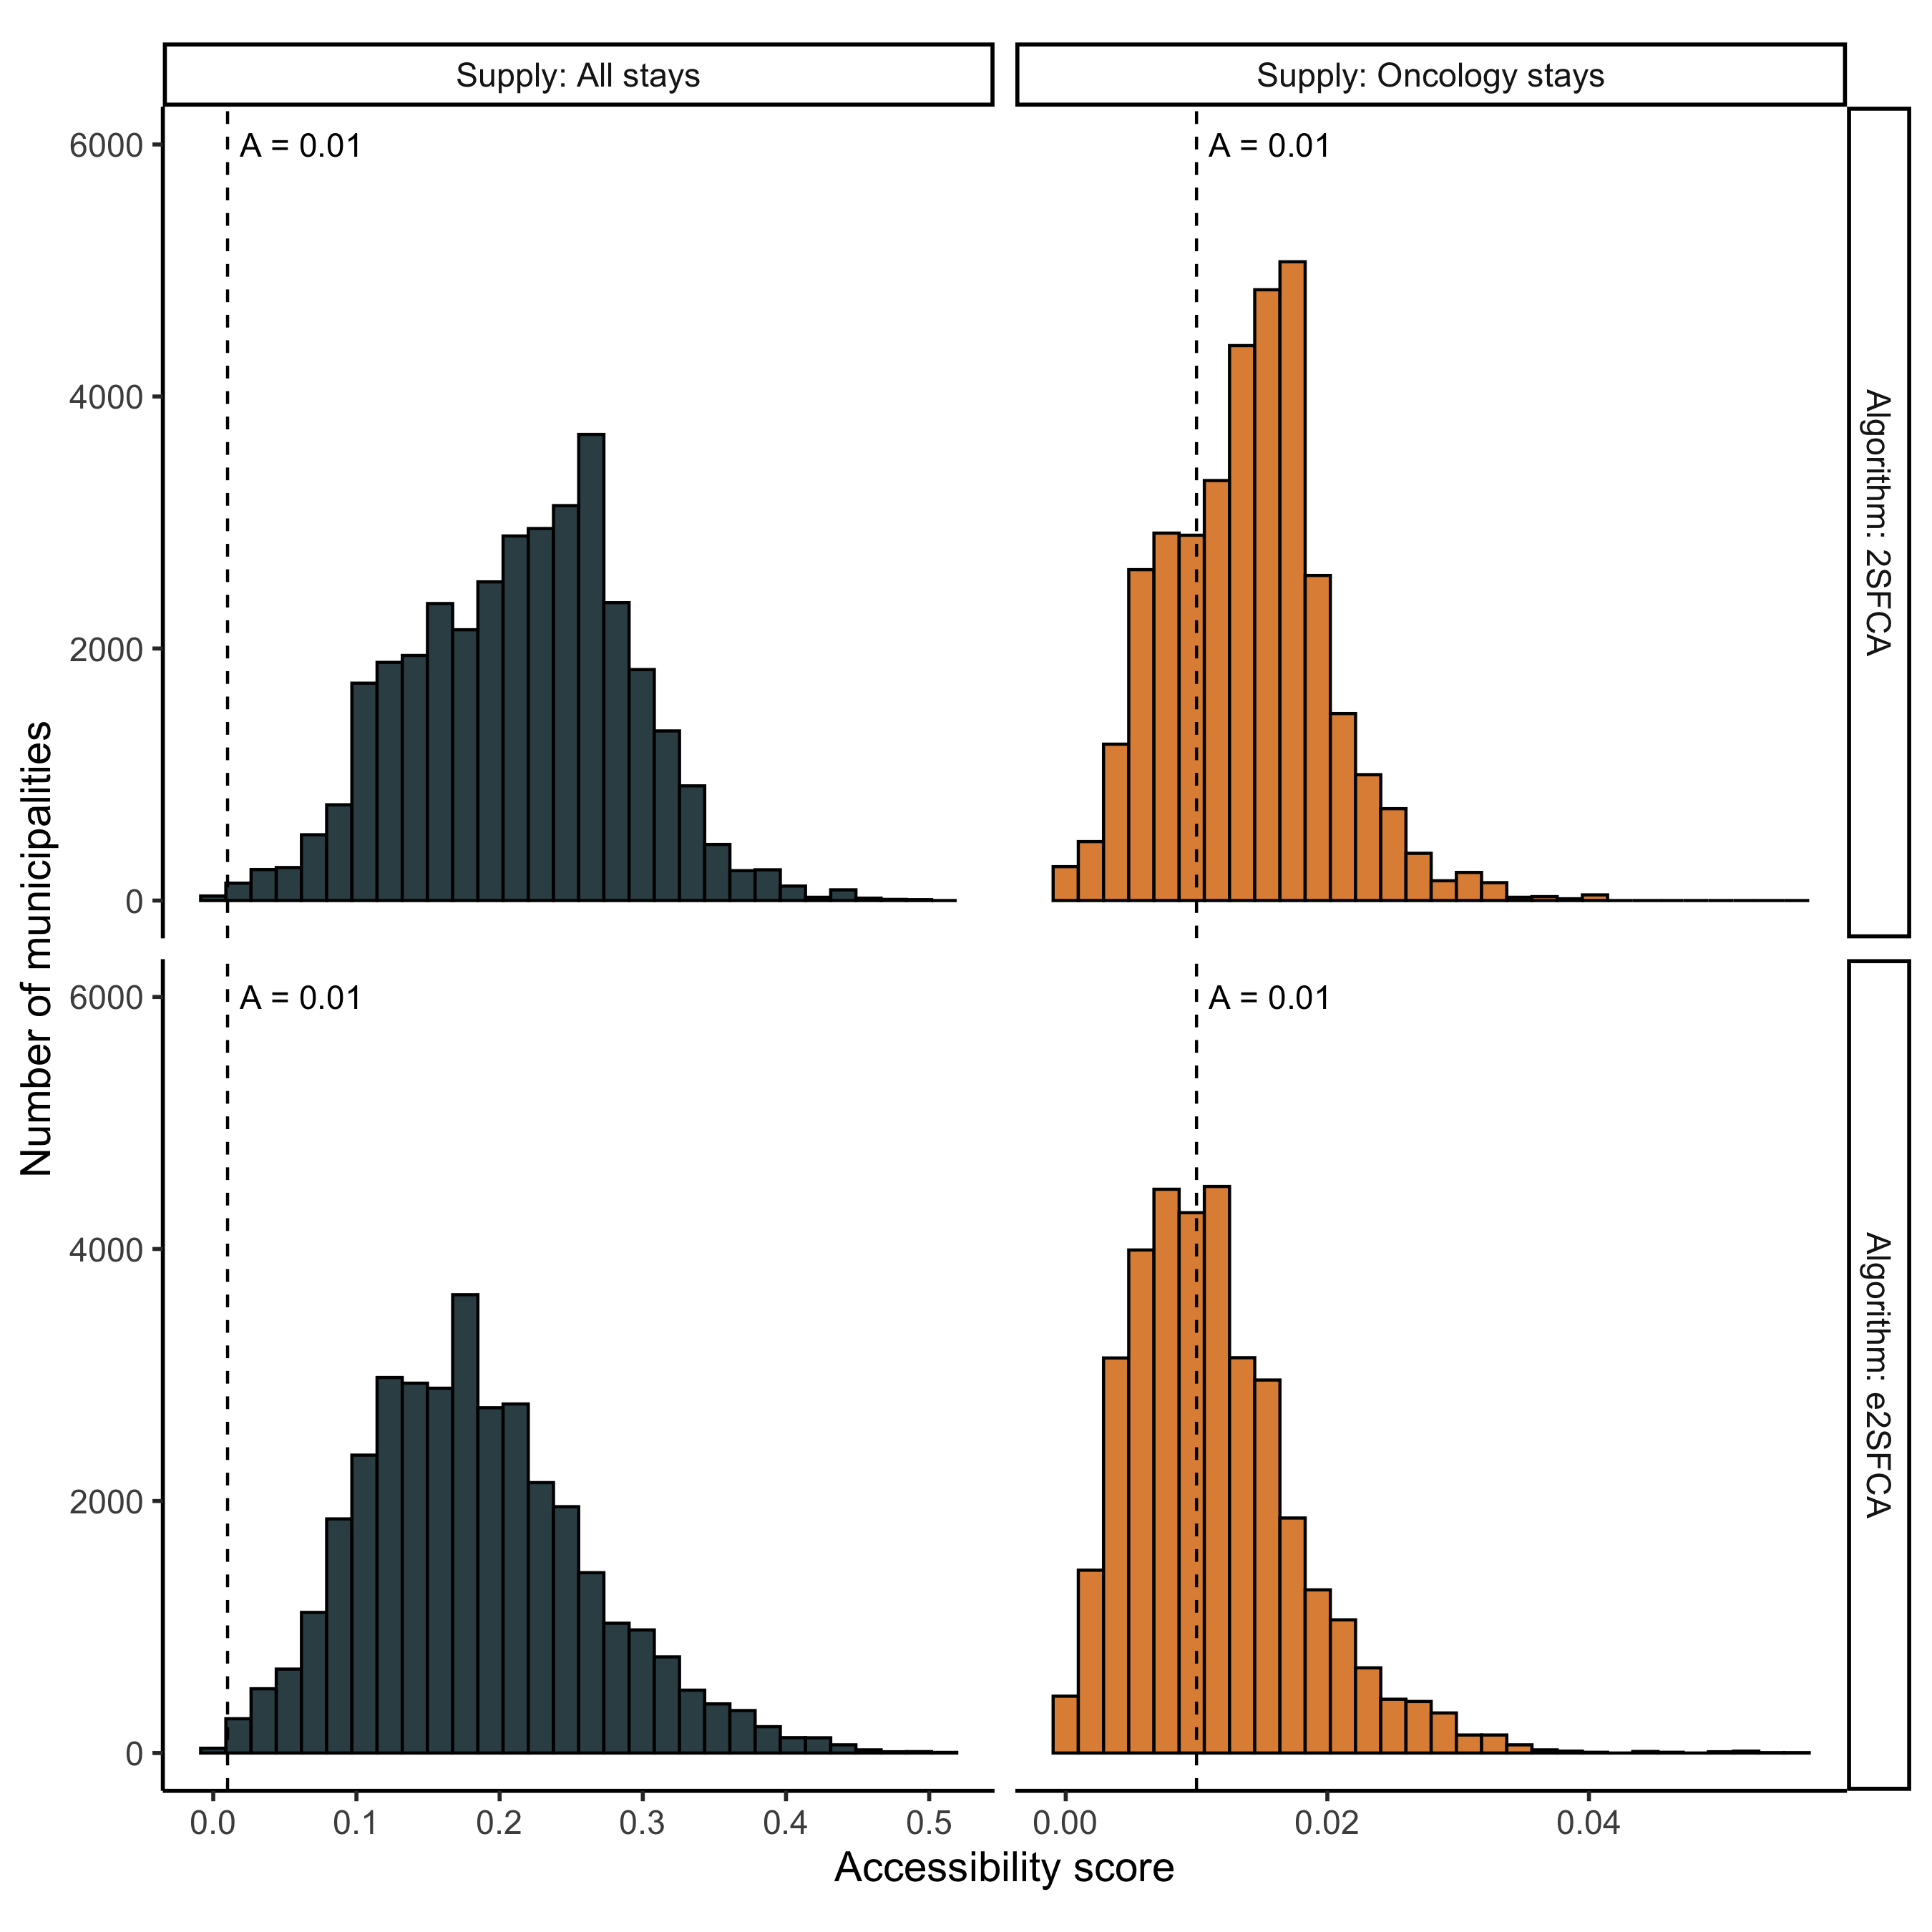
\includegraphics[width=0.7\textwidth]{images/camion/sup_fig5_accessibility_distribution.png}
    \centering
    \caption{ \textbf{Accessibility scores distribution.} The accessibility was
        lower with \ac{e2sfca} because of the weight decay. We also studied the
        influence of the supply variable in the accessibility score. Accessibility is
        much higher if we use the number of \ac{mco} stays as supply, instead of the
        oncology activity. This makes sense since oncology care centers are less common
        and the overall \ac{mco} activity is higher than the oncology activity. }
    \label{fig:accessibility-distribution}
\end{figure}

As we want to compute the accessibility to oncology care centers, we chose $S_u$
to be the oncology activity of a hospital $u$. We define oncology activity as
the sum of the number of medical and surgery stays related to cancer, and the
number of patients with chemotherapy or radiotherapy. A care center with no
oncology activity will have $R_u=0$ and a municipality that solely has access to
this care center u will have $A_i=0$. We use driving duration as travel
impedance metric, and we set the maximum catchment area to a 90-minute drive. In
2018, only 24,152 patients out of 761,057 (3.2\%) had travel duration greater
than 90 minutes for cancer related pathways. This is low enough to consider that
care centers are non-reachable beyond this distance. We divide the catchment
area into 3 intervals: $I_1=(0,30]$ ,$I_2=(30,60]$ and $I_3=(60,90]$. The
associated weights are respectively $W_1=1$, $W_2=0.042$ and $W_3=0.09$. These
sub catchment areas are set based on the cancer pathways travel duration
distributions and validated with medical experts. The weights are the same than
the \ac{e2sfca} paper \cite{luo_enhanced_2009}. For privacy reasons,
municipalities with small populations are grouped in entities called
``geographic codes'' in the \ac{pmsi} database. We decided to compute the
accessibility score for each geographic code and municipalities that are grouped
in the same code will have the same accessibility score.

\section{Results}

The oncology accessibility is unevenly distributed across the country, as
displayed on \cref{fig:accessibility-france}. For better readability, we cut the
accessibility scores into 5 quantiles. Q5 colored in dark green contains the top
20\% accessibility municipalities, and Q1 in light yellow contains the bottom
20\% ones. The lowest accessibility zones are mostly located in the center of
the country and in mountainous regions like the Alps or the Pyrenees. Plot (B)
shows that most of the population (51.6\%) lives in top 20\% accessibility
municipalities, while 6.3\% lives in the bottom 20\% quantile. On map (A), care
centers are displayed as squares, colored by cluster index, and sized by
oncology activity. We see that accessibility is highest near the most
specialized care centers. Indeed, the proportion of care centers from
specialized clusters decreases in lower accessibility quantiles (C). We then
ranked the departments by median accessibility and showed the top-10 and bottom
10 on plot (D). Among the top-5 departments, 4 are in Ile-de-France. Departments
from the bottom-10 are rural or mountainous areas like Lozère and
Alpes-de-Haute-Provence.  We notice disparities within departments as well, as
outlined by the large interquartile range in Hérault or Alpes-Maritimes. On the
contrary, this spread is very narrow in Ile-de-France departments.

\begin{figure}[h!]
    \includegraphics[width=0.9\textwidth]{images/camion/fig2_accessibility_france.png}
    \centering
    \caption{ \textbf{Distribution of the accessibility score computed with the
            \ac{e2sfca}, in metropolitan France.} Plot (A) shows municipalities
        colored by accessibility quantile. The care centers are drawn as
        squares, colored by cluster, and sized by oncology activity. Plot (B)
        shows the total population by accessibility quantile. Plot (C) displays
        the percentage of care centers by cluster by accessibility quantile.
        Plot (D) shows the top 10 and bottom 10 list of the departments, ranked
        by median accessibility. }
    \label{fig:accessibility-france}
\end{figure}

Accessibility score should be put into perspective with population density.
Overall, the denser municipalities have a median accessibility around 0.02.
Municipalities with low population densities have more extreme values.
\cref{fig:accessibility-vs-density} compares accessibility and population
density for three different regions: Provence-Alpes-Cote-d'Azur (A),
Ile-de-France (B), and Bourgogne-Franche-Comté (C). Municipalities are displayed
as squares, colored by accessibility quantile, and sized by population density.
These regions show very different profiles. In Provence-Alpes-Cote-d'Azur (A),
accessibility is essentially low in non-dense municipalities near the Alps.
However, in Bourgogne-Franche-Comté (C), we see dense municipalities with poor
accessibility scores, representing a large proportion of the region. We also
drew similar maps (D, E and F) where municipalities are colored based on the
average travel duration for patients with cancer in 2018. We see that the
average travel time is higher in municipalities with poor accessibility scores.

\begin{figure}[h!]
    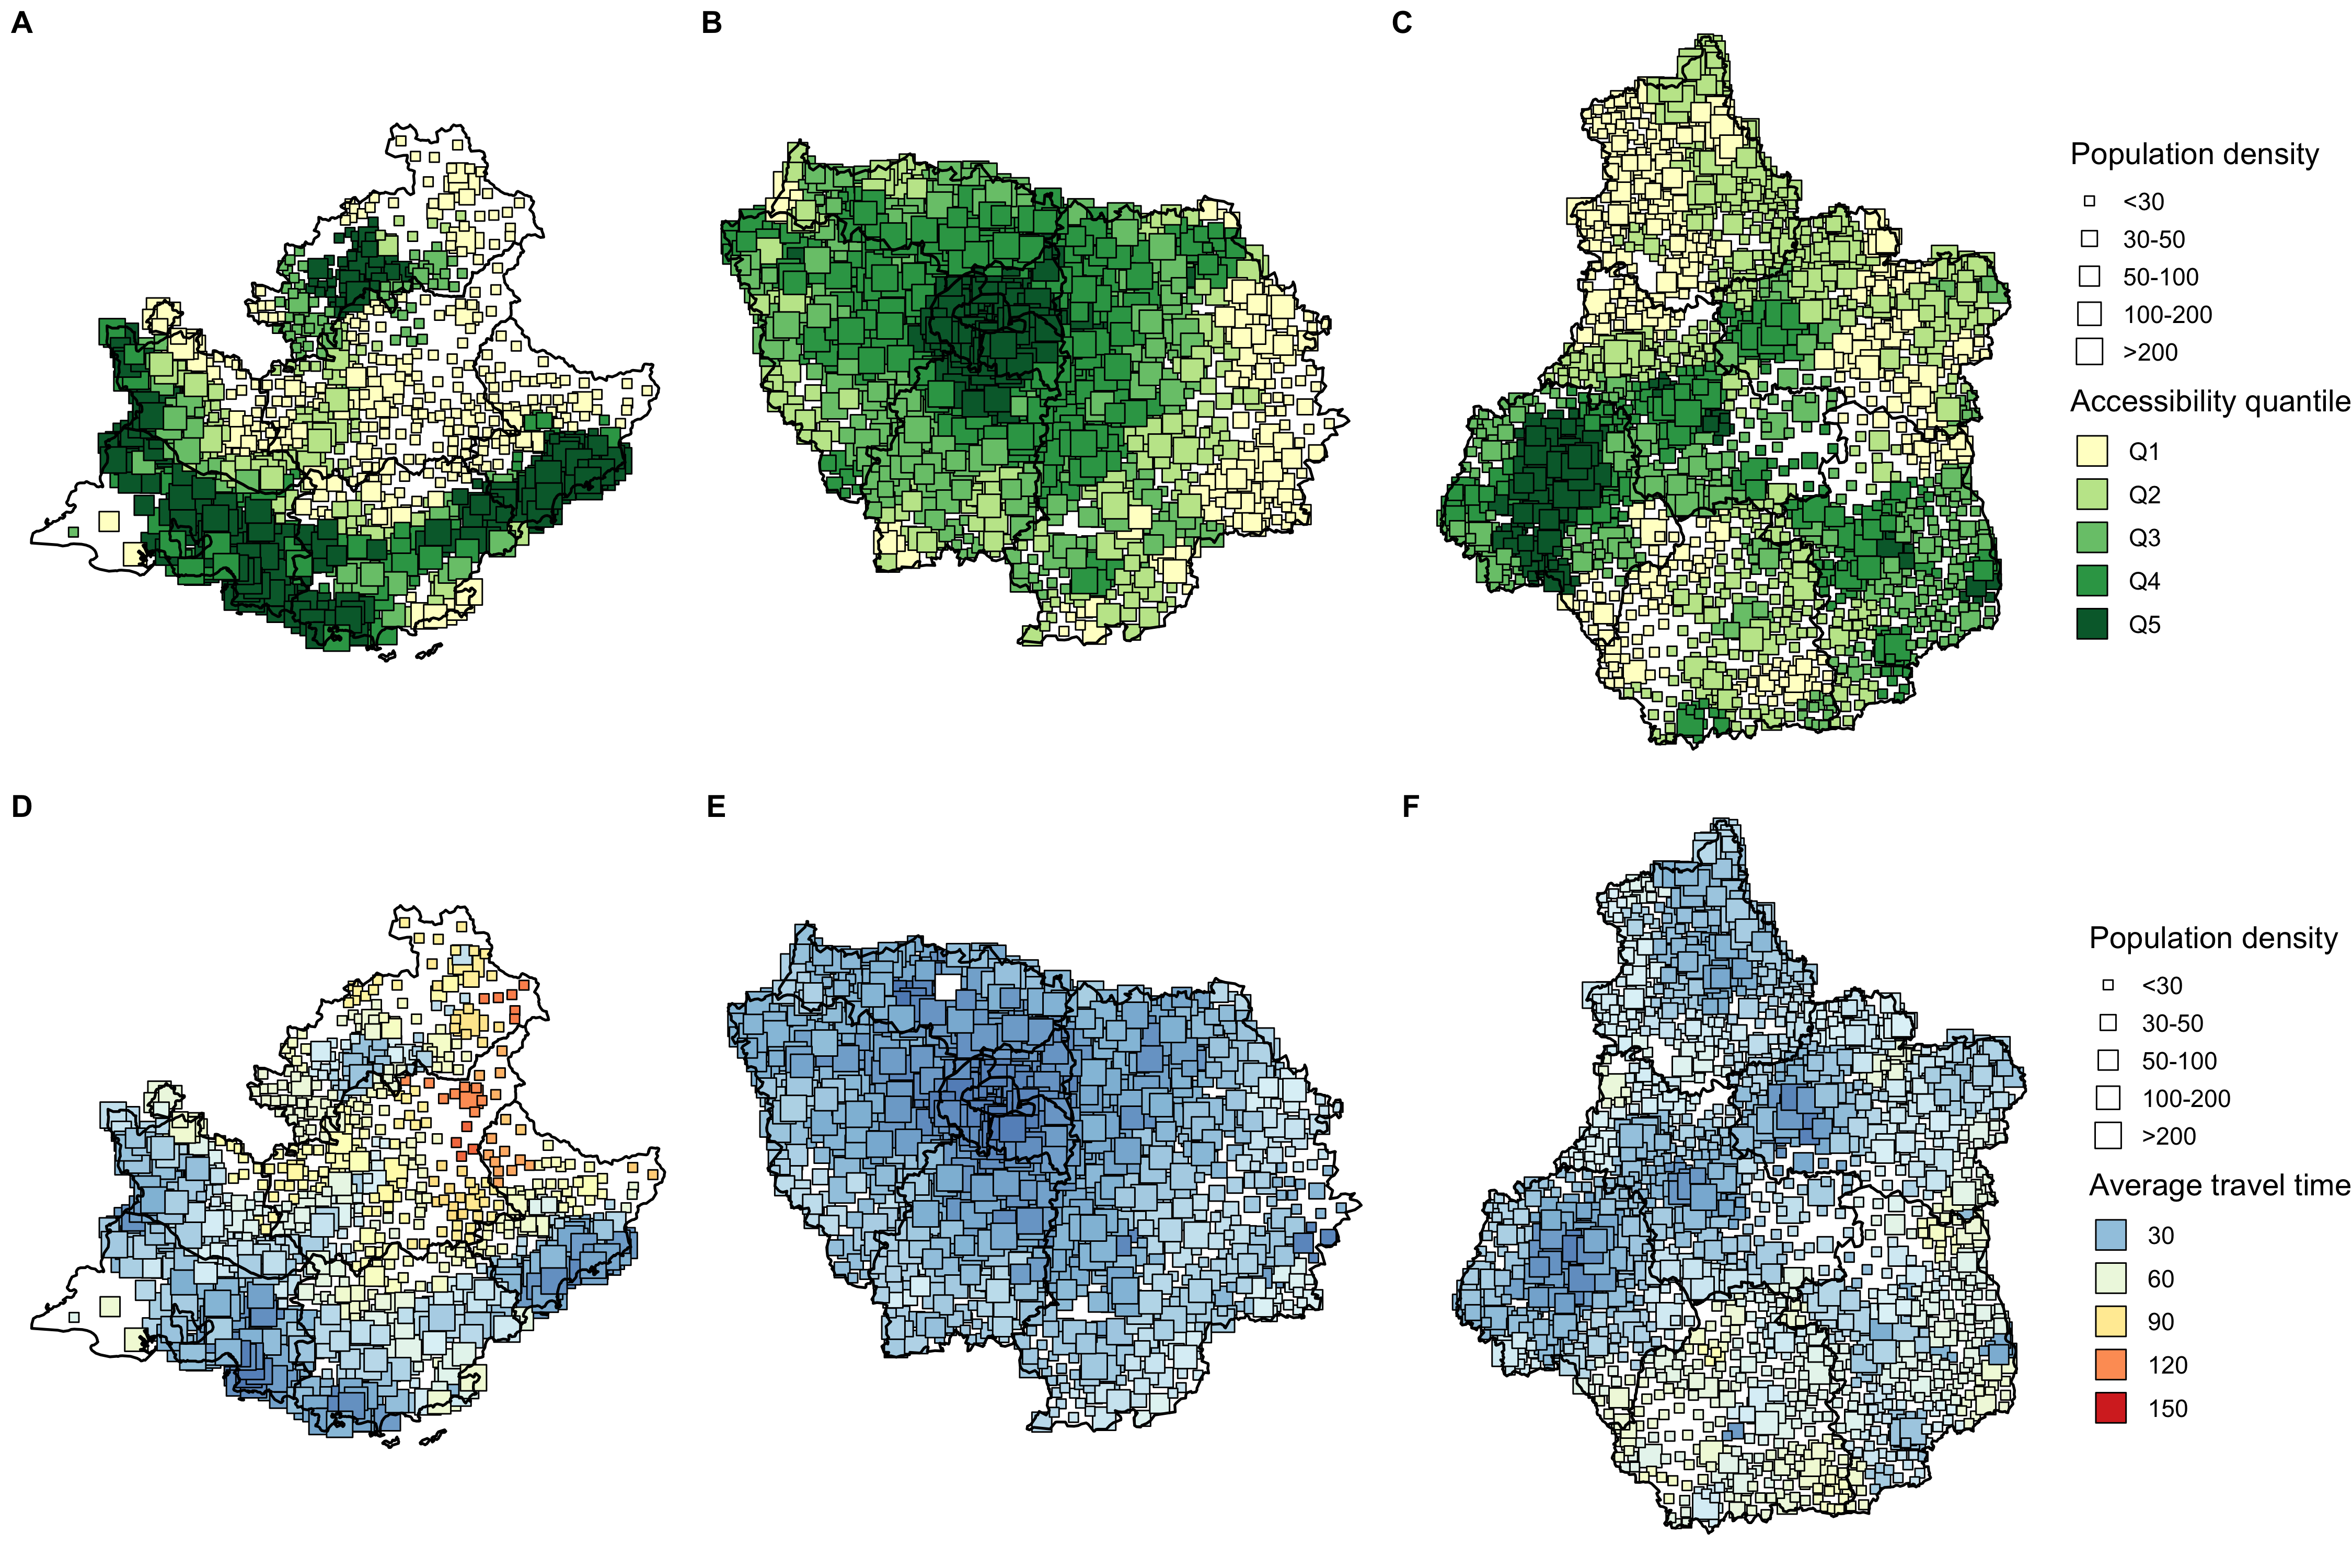
\includegraphics[width=0.9\textwidth]{images/camion/fig3_accessibility_vs_density_scatter_map.png}
    \centering
    \caption{ \textbf{Comparison of population density with accessibility scores
            and patient average travel time for cancer pathways.} Showing results in
        three regions: Provence-Alpes-Cote-d'Azur (A, D), Ile-de-France (B, E)
        and Bourgogne-Franche-Comté (C, F). Municipalities are drawn as squares,
        sized by population density and colored by either accessibility quantile
        (A, B, C) or patient average travel time (D, E, F). }
    \label{fig:accessibility-vs-density}
\end{figure}

Finally, we compared our accessibility score with the department exit ratio, by
municipality. Department exit ratio is defined as the proportion of cancer
patients who visited a care center outside from their department of residence
and was computed using the \ac{pmsi} database. In Provence-Alpes-Cote-d'Azur,
the exit ratio is higher in departments with low accessibility scores and few
oncology specialized care centers, as in Alpes-de-Haute-Provence and
Hautes-Alpes. While the Var department has some oncology centers, exit ratio
remains high since larger care centers are in Marseille and Nice.

\subsection*{Accessibility in Provence-Alpes-Cote-d'Azur region}

We now focus on the region Provence-Alpes-Cote-d'Azur. This region is the far
southeastern on the mainland. The region's population was 5,048 million in 2018.
Its prefecture and largest city is Marseille. The region contains six
departments. Bouches-du-Rhone, Var and Alpes-Maritimes are located on the
coastline and gather the largest cities like Marseille, Nice, or Toulon.
Alpes-de-Haute-Provence, Vaucluse, and Hautes-Alpes are inland departments, with
a majority of rural and mountainous areas. Results are shown on
\cref{fig:accessibility-paca}. By comparing maps (A) and (B), we confirm that
the accessibility is maximum in denser areas of the region. Average patients
travel time are displayed on map (C) and we drew the major roads (primary,
motorway and truck) in red. The road system is well developed on the coast,
rallying the larger cities of the region. However, driving from the rural areas
in the Alps to the major cities is hard, resulting in higher travel times. The
accessibility is unevenly spread within the departments, especially in
Alpes-Maritimes where the distribution is multi-modal (D). There, cities like
Nice and Cannes have large hospitals thus good accessibility, while the northern
areas of the department are mostly mountains. Accessibility is higher in
municipalities with dense populations, for all the departments (E). Finally, the
average travel time decreases when the accessibility score increases. This makes
sense since the accessibility score was computed based on the driving distance
between population locations and care centers. However, it confirms that
patients living in poor accessibility zones effectively travel further to seek
oncology care. In Bouches-du-Rhone, nearly all the municipalities have an
average travel time lower than 30 minutes, while in Alpes-de-Haute-Provence,
average travel times are rarely lower than 60 minutes (F).

\begin{figure}[h!]
    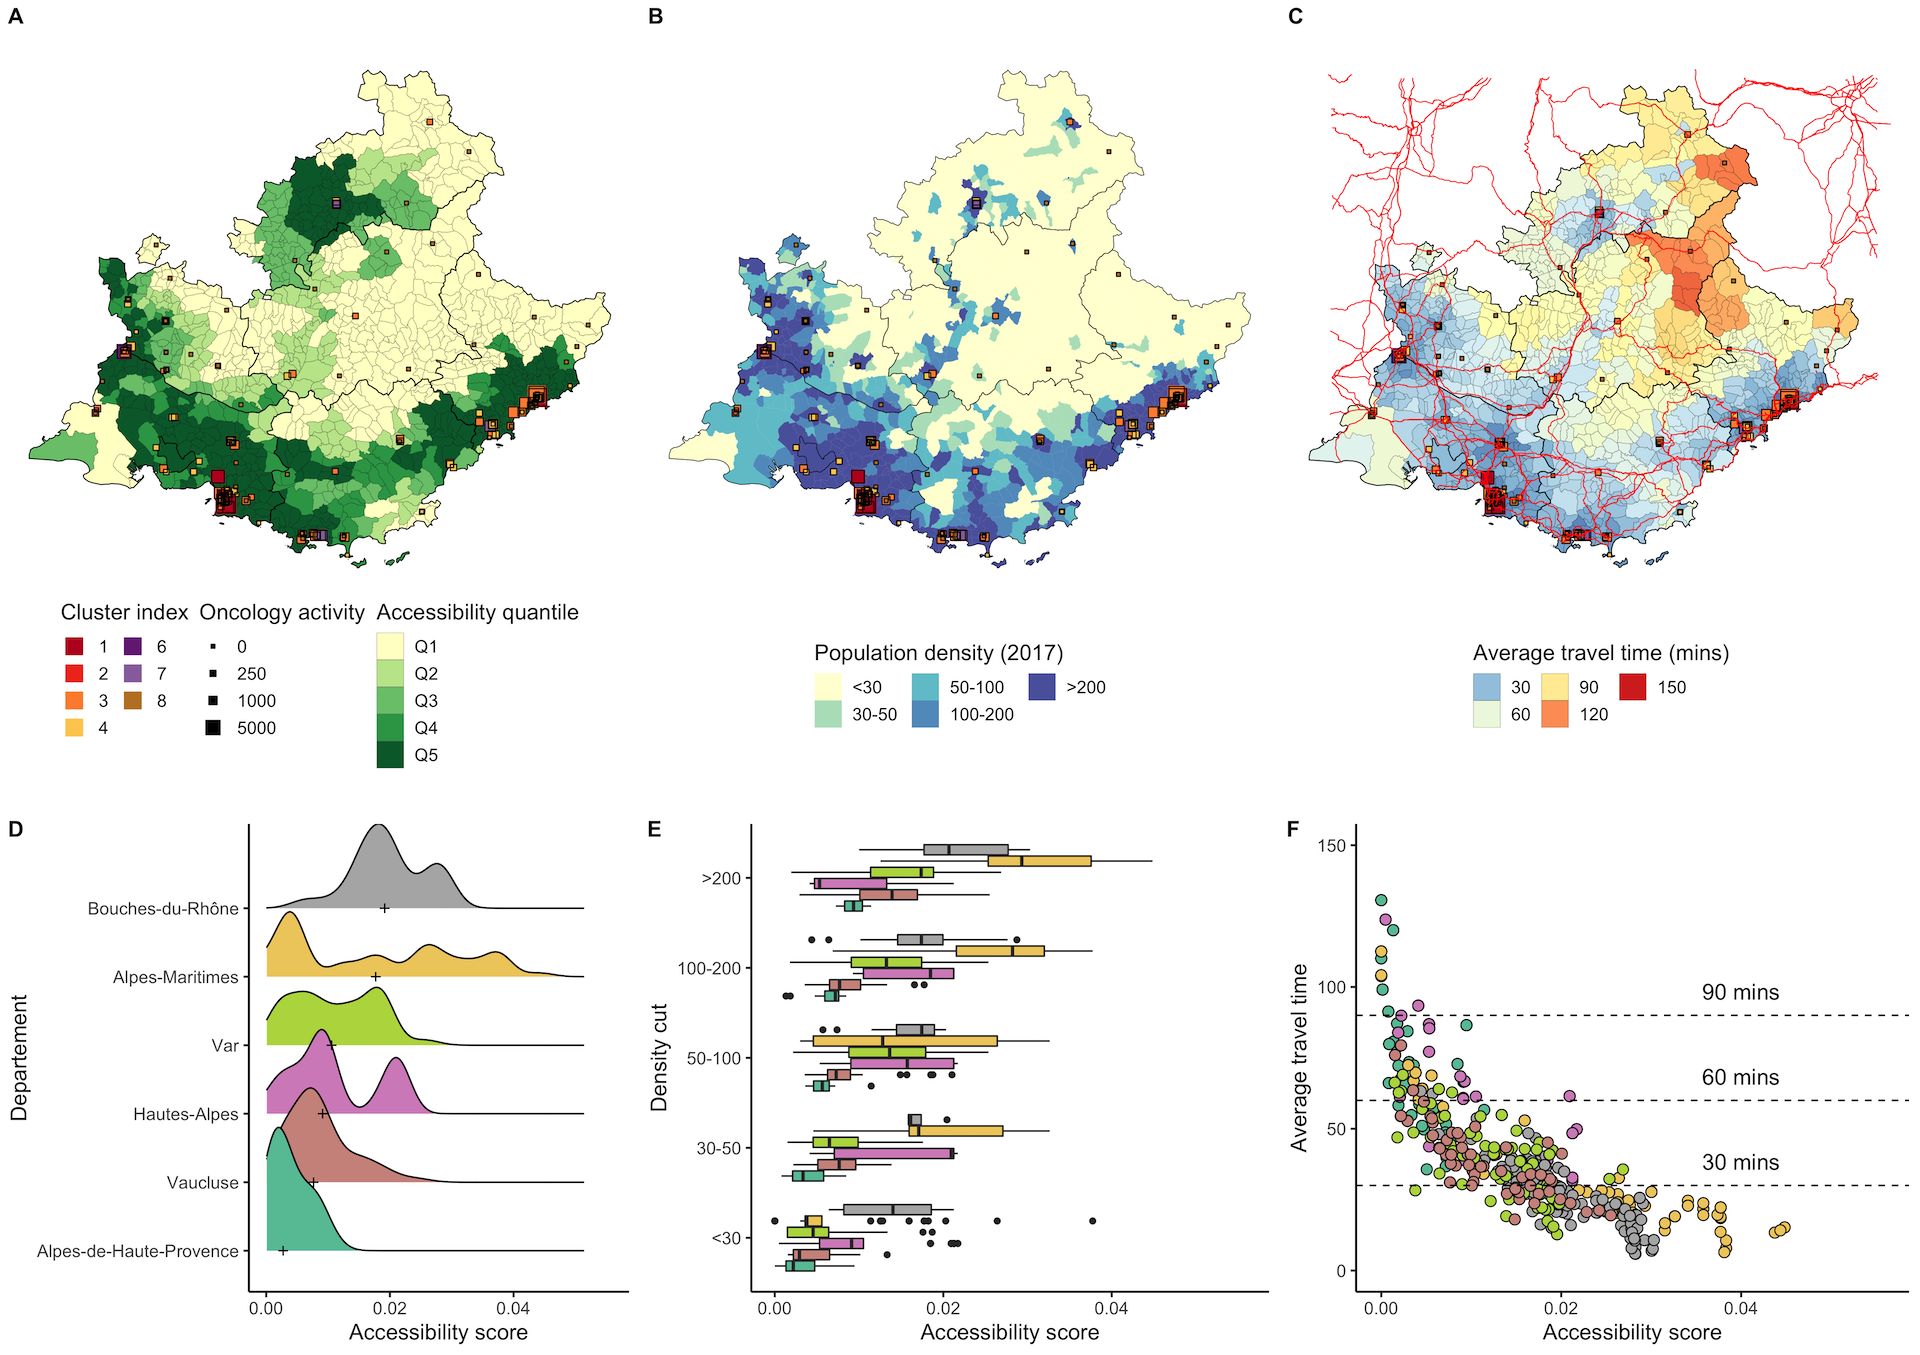
\includegraphics[width=0.9\textwidth]{images/camion/fig4_accessibility_Provence-Alpes-Cote-d'Azur.png}
    \centering
    \caption{ \textbf{Accessibility distribution in Provence-Alpes-Cote-d'Azur
            region.} Map (A) shows the region accessibility distribution per
        municipality. Map (B) displays the population density discretized in 5
        bins. The map on plot (C) displays the average travel time for cancer
        pathways. Large roads (primary, motorway and trucks) are drawn in red.
        Plot (D) shows the accessibility distribution per department of the
        region. Plot (E) shows the accessibility distribution by municipality
        population density and department. Plot (F) compares the accessibility
        score from municipalities with the average travel time for cancer
        pathways. }
    \label{fig:accessibility-paca}
\end{figure}

\subsection*{Accessibility in Pays de la Loire region}

The Pays de La Loire region is located in the west of France. It covers 32,082
km\textsuperscript{2} which makes it the largest region in France, with a
population of 3,806,461 (Insee) in 2019. In the region, one out of two
inhabitants lives in rural areas, compared to one out of three on average in
France. The Pays de la Loire is thus the 4th most rural region behind New
Aquitaine, Brittany and Burgundy-Franche-Comté.  The Pays de La Loire region is
composed of 5 departments. The level of population living in rural communes
varies according to the departments, but 4 departments out of the 5 are
considered rural.  In Vendée and Mayenne, two out of three inhabitants live in
rural areas, in Maine-et-Loire 58\% of the population resides in a rural commune
and in Sarthe 56\%. However, 29\% of the region's population lives in a rural
commune under the influence of a pole, compared to 20\% in an independent rural
commune. The city of Nantes, located in Loire-Atlantique in the east of the
region, is the largest urban area in the region and has 303,382 inhabitants, as
well as 961,521 inhabitants in its urban unit. The region has several cities
with more than 100,000 inhabitants with Le Mans and its 143,325 inhabitants,
Angers (151,520 inhabitants), followed by cities of about 50,000 inhabitants
such as Saint-Nazaire, (68,200 inhabitants) Cholet, (54,200 inhabitants) and
Laval (51,000 inhabitants). The Pays de la Loire has good accessibility with
51\% of its population living in a territory with maximum accessibility and a
low rate of its population living in territories with low or very low
accessibility: 8.3\% of its population resides in an accessibility score zone of
Q2 and only 3.7\% of its population in Q1. Thus, the maps show a good
distribution of accessibility across the territory that varies proportionally
with population density, with low accessibility areas corresponding to areas
with low or very low population density. Travel time is also relatively evenly
distributed across the region, with average travel times of 30 minutes, although
depending on the department, a significant proportion of trips are between 30
and 60 minutes. A very small proportion of territories exceed 60 minutes of
travel time. The territories with longer travel times are located in the Vendée
department, mainly due to the coastal profile of the department and the islands
that make it up, such as the Noirmoutier peninsula or the Ile d'Yeu, where
travel times exceed 90 minutes and 120 minutes respectively.

\begin{figure}[h!]
    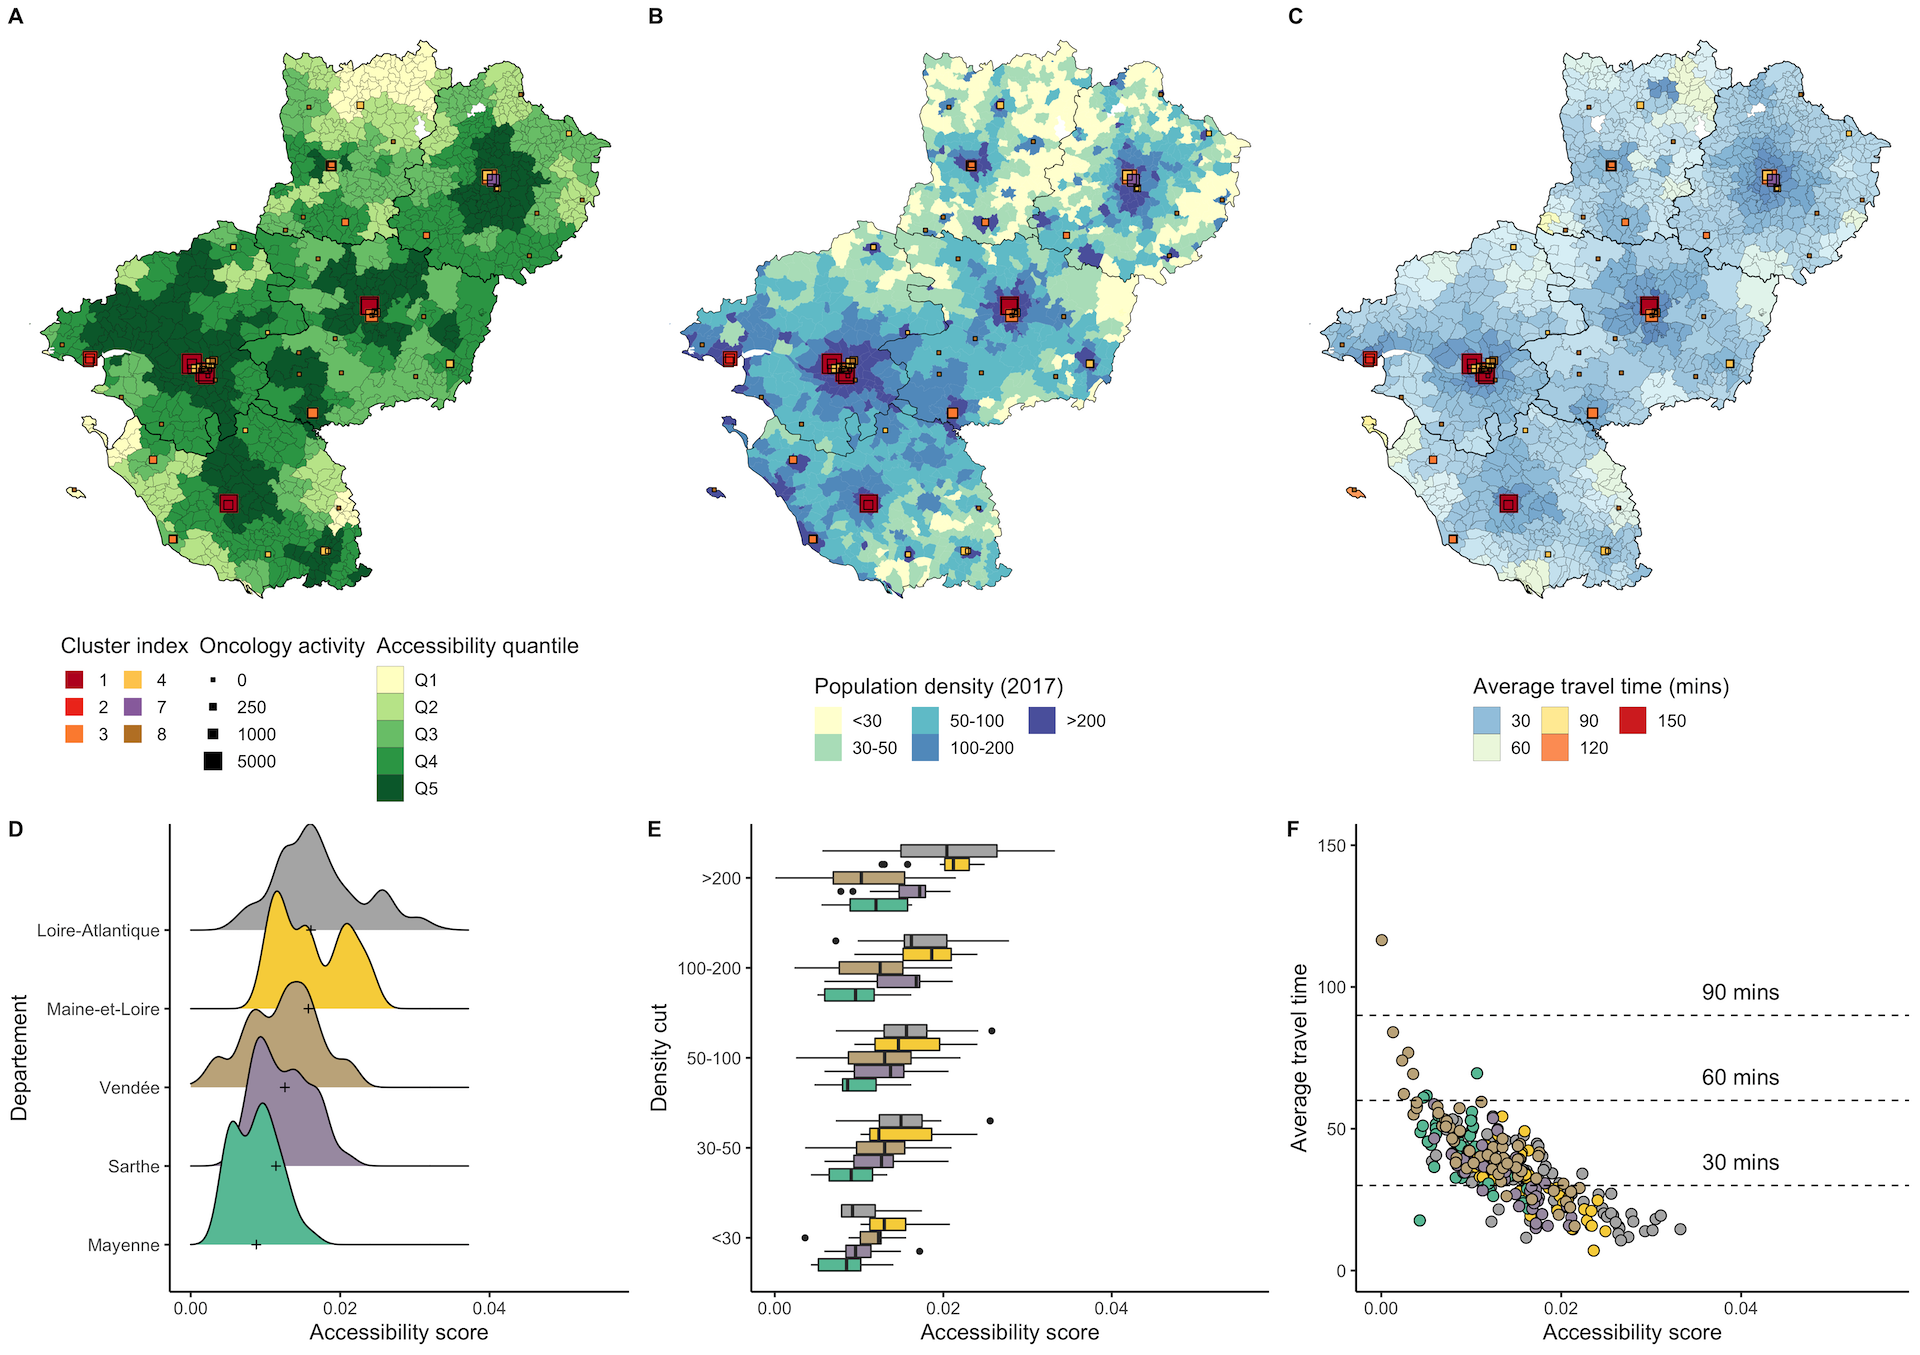
\includegraphics[width=0.9\textwidth]{images/camion/region_accessibility/accessibility_Pays-de-la-Loire.png}
    \centering
    \caption{
        \textbf{Accessibility distribution in Pays-de-la-Loire.} The accessibility distribution
        in this region is high, and the amount of municipalities with Q5 accessibility
        score is very low. The median accessibility is the highest in Loire-Atlantique
        department, especially around Nantes; or in Maine-et-Loire near Angers. The
        lowest median accessibility is in Mayenne, where the main city is Laval. The
        accessibility is lower in the northern part of this department, where the
        population density decreases compared to the rest of the region.
    }
\end{figure}

\subsection*{Accessibility in Occitanie region}

The Occitanie region is located in the South of France. It covers 72,724 km² for
a population of 5,933,185 (Insee) in 2019, for a population density of 81.6
inhabitants/km² the 6th least dense region in metropolitan France. The rural
territory in Occitanie represents 90\% of the territory, mainly present in the
mountain areas of the Massif Central and Pyrenees. The urban space is mainly
found along the coast and in the Garonne basin. 39\% of the population lives in
rural areas, i.e. 2.9 million inhabitants, and 9 of the 13 departments are
considered rural. However, Occitanie is a largely urbanized territory with
numerous urban centers in each department, the main metropolises being Toulouse
and Montpellier. This region is the 5th most urbanized region of the metropolis
and has more than fifty urban units of at least 10,000 inhabitants with several
cities exceeding 70,000 inhabitants (Tarbes, Montauban, Albi). 4.4 million
people live in the urban units, representing 76\% of the population. Occitanie
is composed of 13 departments. Three departments are among the most urbanized in
the province and therefore have a strong demographic weight: Hérault (89\% of
the population residing in an urban unit), Pyrénées-Orientales (88\%) and
Haute-Garonne (87\%). The Hérault department includes the city of Montpellier,
but also Béziers, Sète and many small urban areas. The Haute Garonne includes
the city of Toulouse, the fourth most populated commune in France (493,465
inhabitants) and with its rural areas are under strong pole influence.  The Lot,
Lozère and Gers are the least urbanized in France, with less than 40\% of the
population living in urban areas.

In this region, accessibility is not uniform across the territory. The areas
with the highest accessibility scores are concentrated in the large urban areas
and their catchment areas, notably in the center of the region around the city
of Toulouse and Montauban in the Garonne basin, as well as along the coastline
in the east of the region around the cities of Nîmes, Montpellier, Béziers,
Narbonne and Perpignan. Also, if the most densely populated areas have a good
level of accessibility, it can be seen that some medium-sized cities in the
Occitanie region lack a good level of accessibility and even have low
accessibility. This is particularly pronounced in the rural departments of the
region (Lot, Gers and Lozère), as well as in Aude, Ariège and Hautes-Pyrénées.
Indeed, many urban units have a low accessibility score (Q2) such as Auch
(25,527 inhabitants) in the Gers, Foix (12,310 inhabitants) and Pamiers (29,340
inhabitants) in the Ariège, Rodez (47,868 inhabitants) in the Aveyron with a
score of Q2/Q3, Cahors (24,279 inhabitants) in the Lot. Many areas of the region
have long travel times of around 90 minutes if not 120 minutes on average. This
is particularly true along the border with Spain, which is characterized by its
mountainous terrain. However, the Gers, Lot, Lozère, Aveyron and Hérault regions
have average travel times of around 90 minutes. These high travel times are
mainly associated with sparsely populated areas, although in the Hautes-Pyrénées
department, average travel times of 90 minutes can be seen around the urban unit
of Bagnères de Bigorre (13,213).

\begin{figure}[h!]
    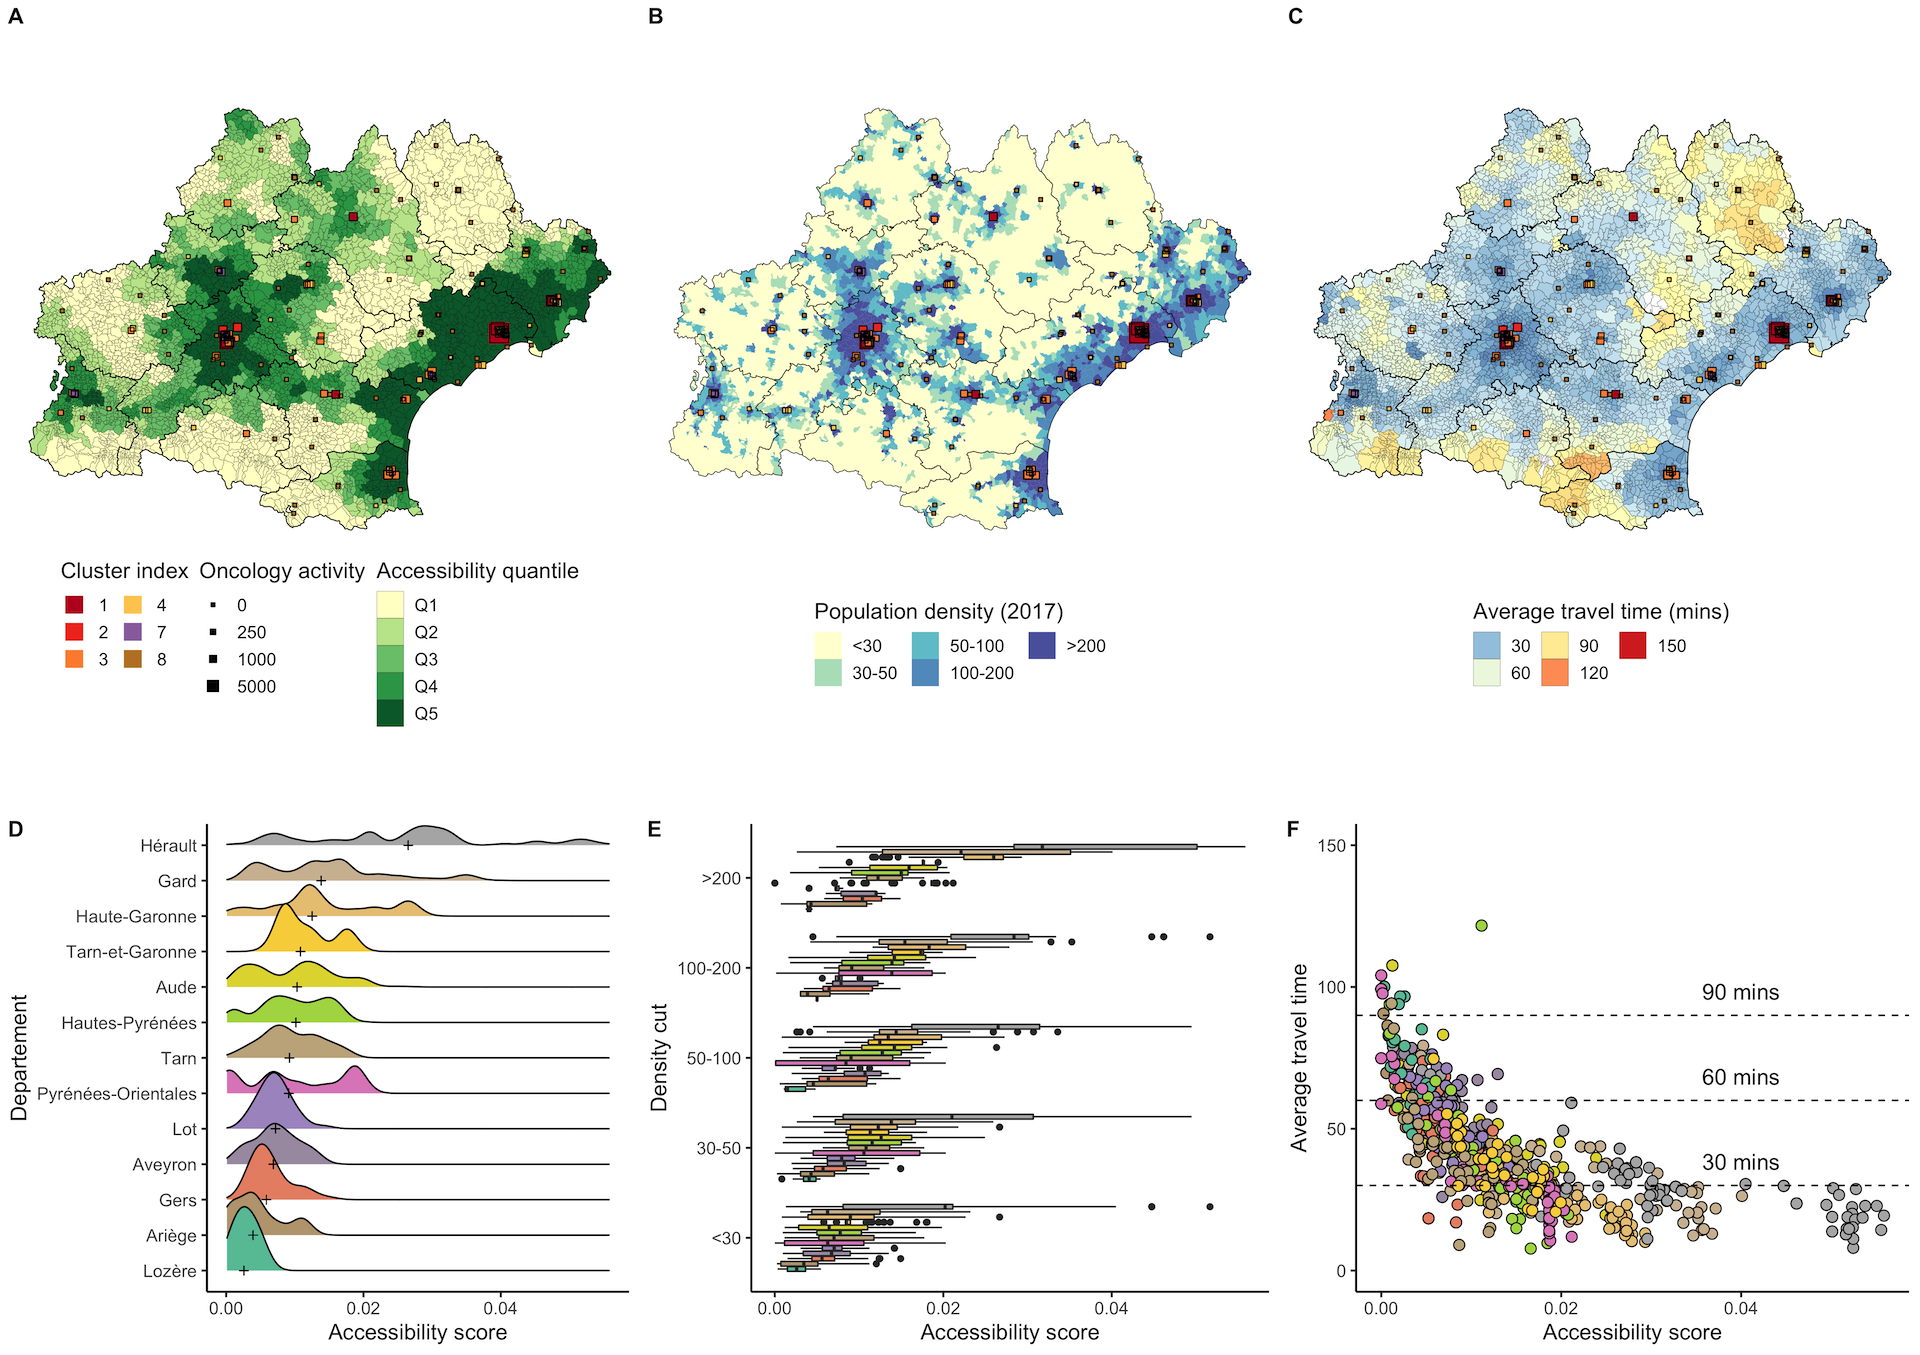
\includegraphics[width=0.9\textwidth]{images/camion/region_accessibility/accessibility_Occitanie.png}
    \centering
    \caption{
        \textbf{Accessibility distribution in Occitanie.} The areas with the highest accessibility scores are concentrated in
        the large urban areas and their catchment areas, notably in the center of the
        region around the city of Toulouse and Montauban in the Garonne basin, as well
        as along the coastline in the east of the region around the cities of Nîmes,
        Montpellier, Béziers, Narbonne and Perpignan.
    }
\end{figure}

\subsection*{Accessibility in Nouvelle-Aquitaine region}

The Nouvelle-Aquitaine region is located in the southwest of France. It covers
an area of 84,036 km\textsuperscript{2} which makes it the largest region in
France, with a population of 6,010,289 (Insee) in 2019. The region is the third
most rural region of France with half of its inhabitants living in a rural
commune. The share of population in rural autonomous is significant compared to
the national average but is similar to that of Brittany or
Burgundy-Franche-Comté. Among the twelve departments of Nouvelle-Aquitaine , ten
are predominantly rural, and two are predominantly urban: Gironde (71\% of the
population living in an urban commune) and Pyrénées-Atlantiques (62\%).
Nouvelle-Aquitaine is composed of 12 departments. The region's main metropolis,
Bordeaux, with 260,958 inhabitants and 986,879 inhabitants in its urban unit, is
located in the west of the region in the Gironde department. The region includes
several intermediate cities with more than 70,000 inhabitants such as Limoges
(130,876), Poitiers (89,212), Pau (75,627), La Rochelle (77,205), Mérignac
(72,197), Pessac (65,245).

We notice accessibility disparities in this region. The areas with the highest
accessibility scores are mainly located around the above-mentioned large and
intermediate cities. Also, the areas with accessibility scores Q1 and Q2 are
mainly located in territories with low or very low population density.
Similarly, the Nouvelle-Aquitaine region seems to provide relatively widespread
access to cancer care for its population. Indeed, 56\% of its population is
located in a zone with a maximum accessibility score of Q5, and 21.1\% in a zone
with a very good accessibility score of Q4. This leaves a smaller share of the
population in areas of low accessibility (8.4\% in Q2) and very low
accessibility (6.3\% in Q1). The average travel time is well distributed over
the territory, with a majority of the territory covered by travel times between
30 and 60 minutes. It can be seen, however, that part of the territory has a
good share of trips of less than 30 minutes (on average e 15 minutes) even in
areas with average accessibility (score 0.2). A clear correlation can be seen
between accessibility score and average travel time, with longer travel times in
areas with low accessibility scores, but consequently less densely populated
territories. The Landes and Lot-et-Garonne are the departments with the highest
number of trips exceeding 60 minutes.

\begin{figure}[h!]
    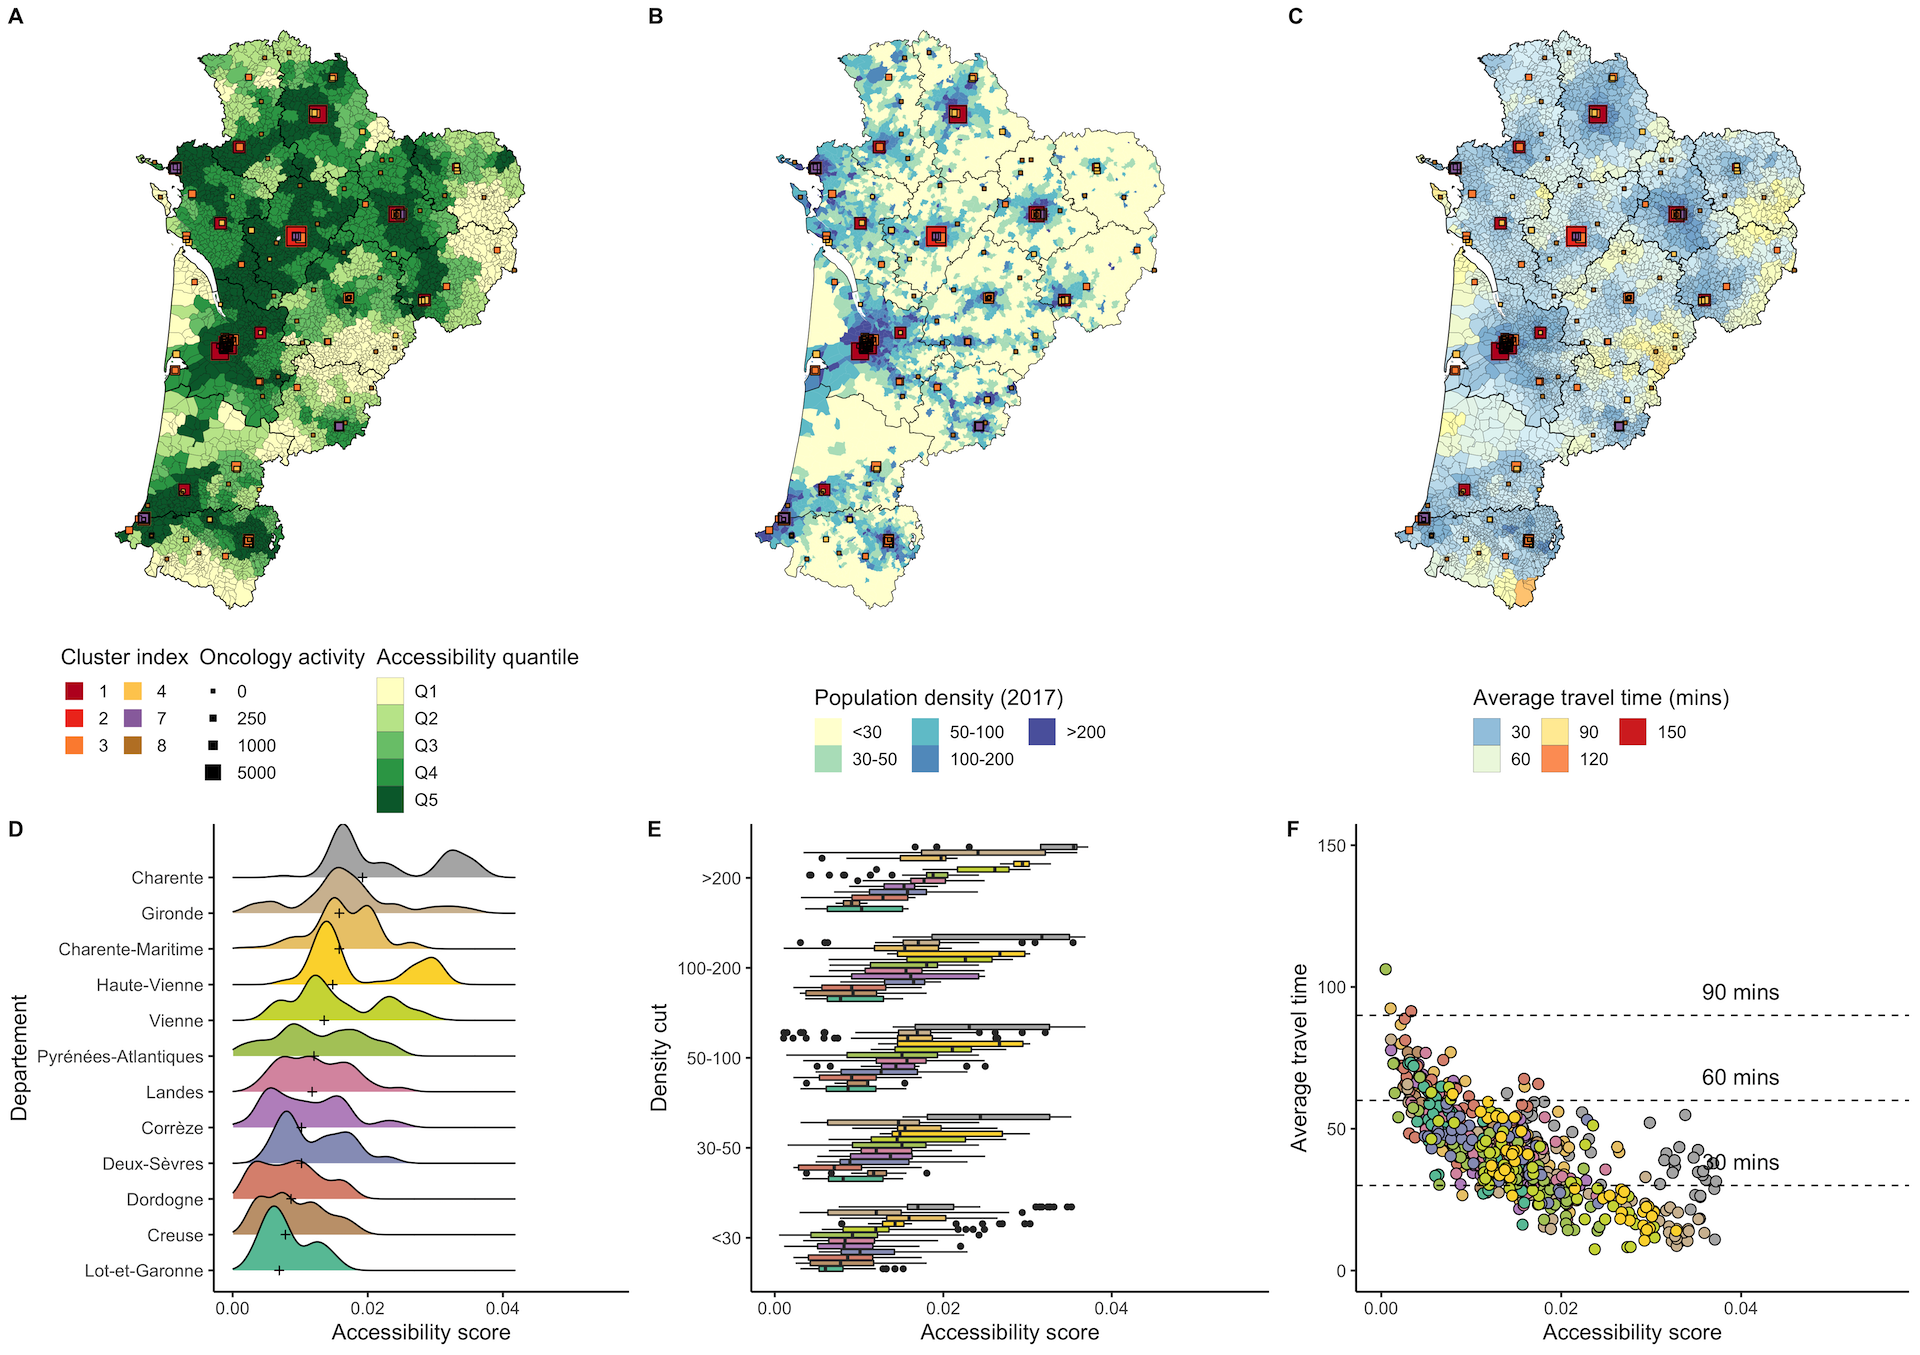
\includegraphics[width=0.9\textwidth]{images/camion/region_accessibility/accessibility_Nouvelle-Aquitaine.png}
    \centering
    \caption{
        \textbf{Accessibility distribution in Nouvelle-Aquitaine.}The areas with the highest accessibility scores are mainly located around the
        above-mentioned large and intermediate cities. Also, the areas with
        accessibility scores Q1 and Q2 are mainly located in territories with low or
        very low population density. The Nouvelle-Aquitaine region seems to
        provide relatively widespread access to cancer care for its population.
    }
\end{figure}

\subsection*{Accessibility in Normandie region}

The Normandie region is located in the north-east of France. It covers 29,905
km² with a population of 3,325,032 inhabitants (Insee) in 2019. The Normandie
region remains a fairly rural region with half of its inhabitants living in a
rural commune (49\% compared to 40\% in the rest of France). The population
living in a rural commune is clearly in the majority in Orne in the south of the
region (73\%), Manche in the west (68\%) and Eure in the east (62\%). However,
more than half of the rural communes are not under the influence of a hub.
Normandie is composed of 5 departments. The department of Seine-Maritime in the
northeast of the region has two of the largest urban units in the region with
more than 200,000 inhabitants: Rouen the most populous with 112,321 inhabitants
and 471,893 in its urban unit as well as Le Havre with 172,366 inhabitants and
233,414 in its urban unit. The third urban unit of more than 200,000 inhabitants
in the region is Caen with 206,973 inhabitants in its urban unit, located in
Calvados. Normandie presents a rather average accessibility in terms of
population density and accessibility ratio since 30.9\% of its population lives
in the best accessibility score almost equivalent to the percentage of
population living in a territory with a Q3 score of 28.3\%. Only 10.3\% of its
population lives in accessibility level Q1 and 9.2\% in Q2.


We notice that the accessibility score is unevenly distributed. Although the
areas with low or very low population density are the most affected by a low
accessibility score of Q1 or Q2, we can still observe a fairly homogeneous
distribution of the population on the territory, especially in the areas far
from the urban units, and an accessibility that remains fairly low around Q2.
The department of Calvados has the best distribution of accessibility over its
entire surface. Whereas Orne, which is the most rural department in Normandie,
has an accessibility score of Q1 except around the urban unit of Argentant. The
same is true for the department of La Manche, which includes many areas of the
territory with an accessibility score of Q1 or especially Q2 despite a higher
population density, notably around the city of Cherbourg-Octeville and its
surroundings with an accessibility score of Q3 or even Q2 for a city that
nevertheless counts 35,545 and 81,423 in its urban unit (Figure 24). The average
travel time is well distributed over the territory, with the majority of the
territory covered by travel times of 30 minutes on average and below 60 minutes.
It can be seen that the majority of trips in the departments of Seine-Maritime
and Calvados are under 30 minutes, particularly in Calvados, unlike the
department of Orne, the only department in the region whose trips are slightly
over 60 minutes but still under 90 minutes.

\begin{figure}[h!]
    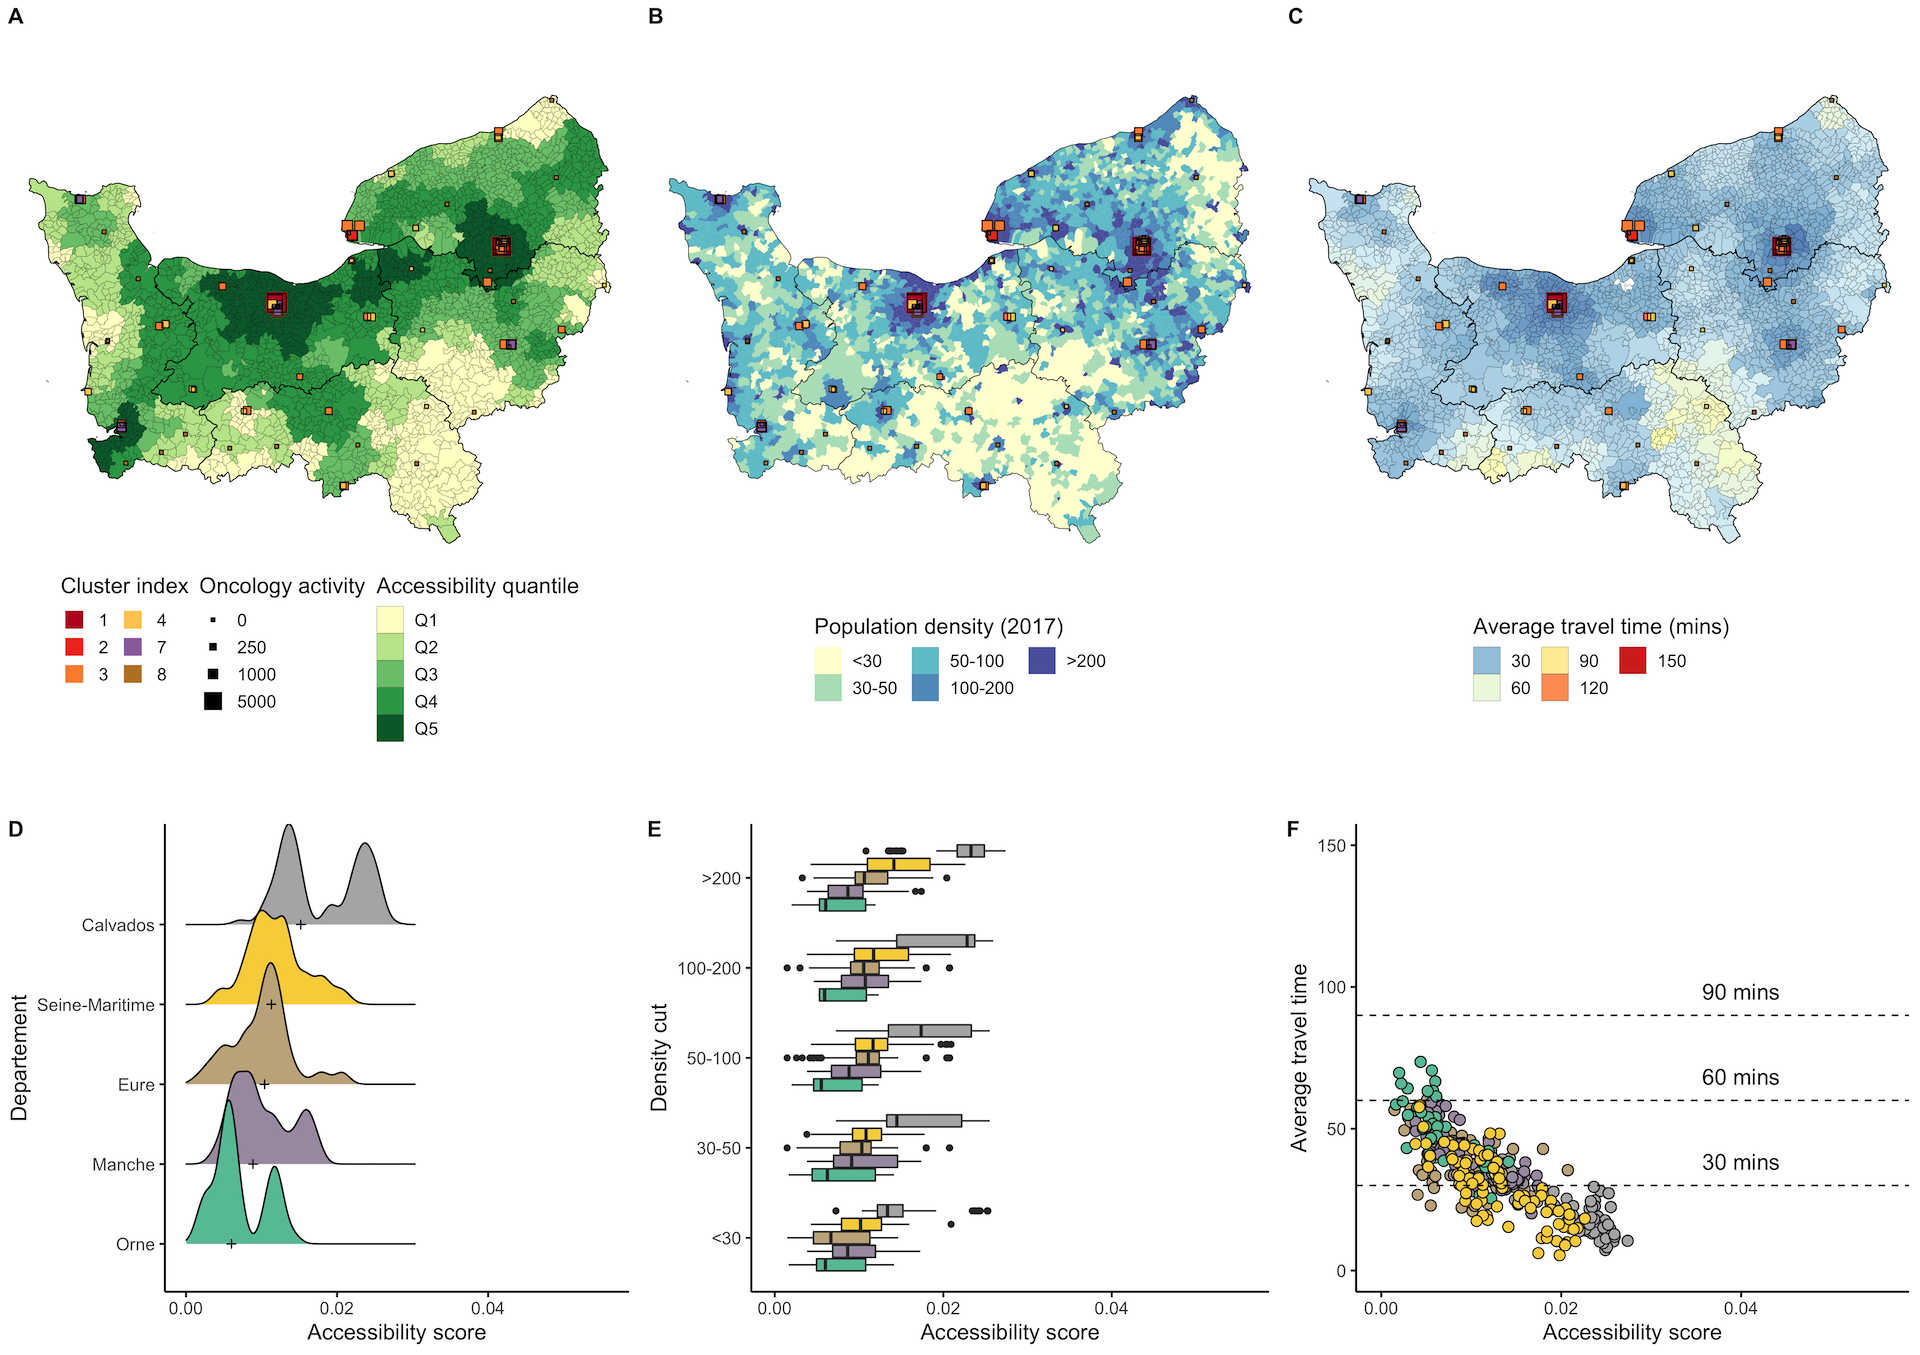
\includegraphics[width=0.9\textwidth]{images/camion/region_accessibility/accessibility_Normandie.png}
    \centering
    \caption{
        \textbf{Accessibility distribution in Normandie.}
    }
\end{figure}

\subsection*{Accessibility in Île-de-France region}

The Île-de-France (IdF) region is located in the center north of France. This
one covers 12,012 km\textsuperscript{2} for a population of 12,213,447 (Insee)
in 2018. The IdF region is the most populated and dense of metropolitan France.
Only 5\% of the population lives in a rural commune, for the 671 rural communes
cover 59\% of the IdF territory. The majority of rural communes (85\%) are under
the influence of Paris. Île-de-France is composed of 8 departments, 4
departments in the inner suburbs and 4 departments in the outer suburbs. It is a
special region because it includes the French capital, Paris, the leading French
city in terms of demography and population density with 2,175,601 inhabitants in
2021. The city of Paris is also home to many specialized health establishments.
The rural communes are far from the influence of Paris and are mainly located in
the departments of the outer suburbs, three quarters of which are in
Seine-et-Marne. The most rural and least dense areas are therefore mainly
located in the east of the region, particularly along the border to the east of
the Seine-et-Marne department.

Île-de-France has good accessibility over the vast majority of its territory.
Indeed, 63.8\% of the population of IdF is located in an area with a maximum
accessibility score, and almost no population is located in an area with a
minimum accessibility score Q1 or even Q2. Also, although only 9\% of the
territory's surface is identified as having a Q5 score and 15\% as having a Q1
score, the minimum accessibility zones are not very densely populated, which
only affects a very small part of the region's population. Indeed, we observe
that the only areas with a Q1 score are located in the eastern part of the
region in the Seine-et-Marne department where the population density is very
low. Moreover, travel time is uniform throughout the region with a very good
level of travel time limited to an average of 30 minutes. The Ile-de-France
region does not suffer from accessibility difficulties at any level for cancer
treatments, regardless of location in the territory.

\begin{figure}[h!]
    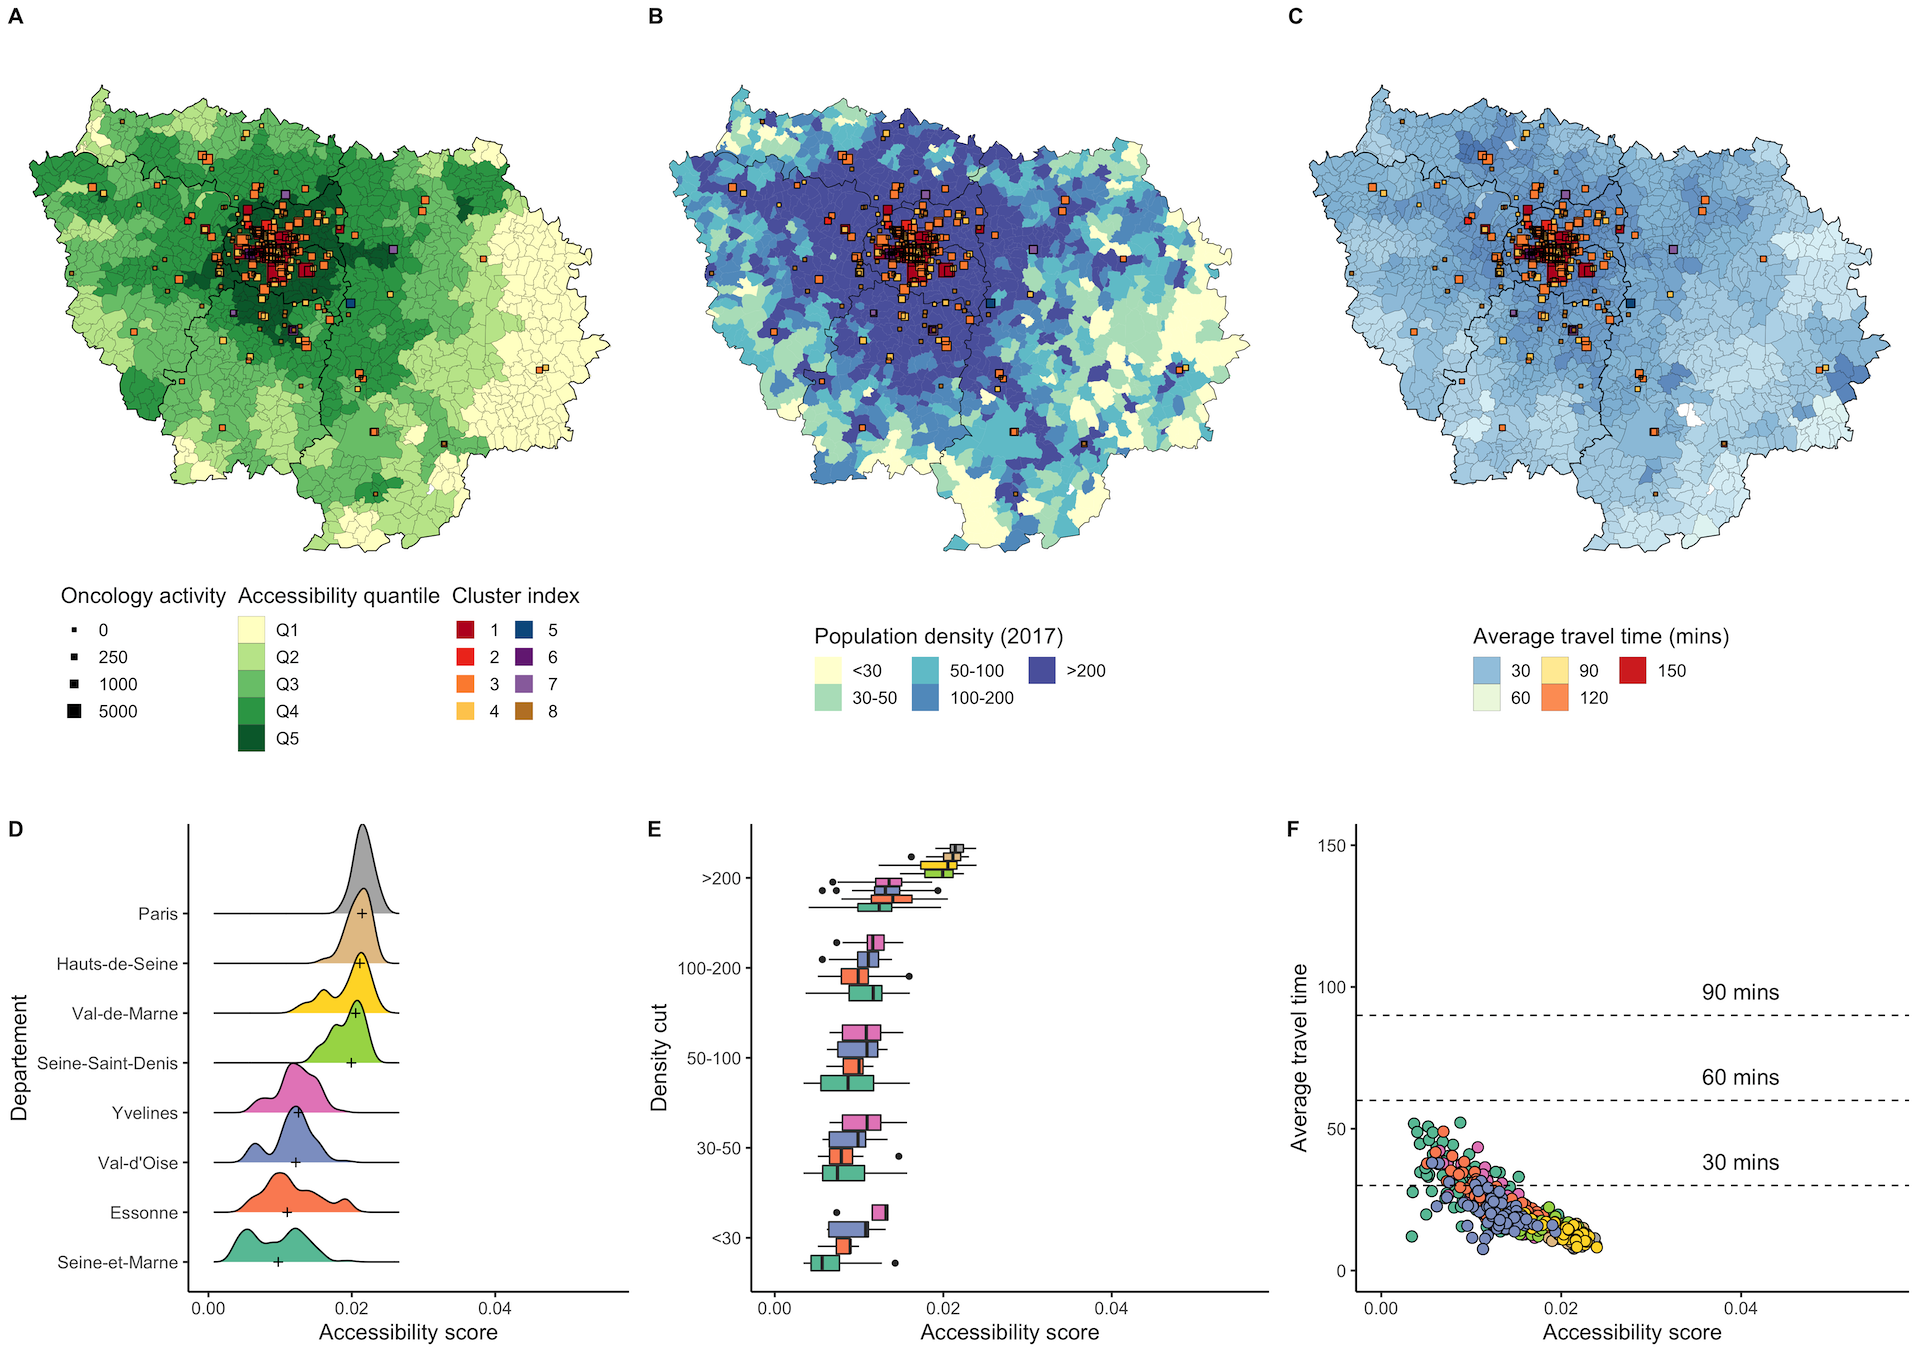
\includegraphics[width=0.9\textwidth]{images/camion/region_accessibility/accessibility_Ile-de-France.png}
    \centering
    \caption{
        \textbf{Accessibility distribution in Ile-de-France.}Île-de-France has good accessibility over the vast majority of its territory.
        Indeed, 63.8\% of the population of IdF is located in an area with a maximum
        accessibility score, and almost no population is located in an area with a
        minimum accessibility score Q1 or even Q2. Also, although only 9\% of the
        territory's surface is identified as having a Q5 score and 15\% as having a Q1
        score, the minimum accessibility zones are not very densely populated, which
        only affects a very small part of the region's population.
    }
\end{figure}

\subsection*{Accessibility in Hauts-de-France region}

The Hauts-de-France region is located in the north of France. It covers
31,948km² for a population of 6,005,000 (Insee) in 2019, or 9\% of the
metropolitan population. The region has retained a strong industrial footprint.
It is the second most urbanized region after Ile de France with 89\% of its
population living in a large urban area. However, 83\% of the region's
municipalities are considered rural (including autonomous rurality and rurality
under the influence of a pole in a peri-urban area), with 29\% of the region's
population living in a so-called rural municipality. The Hauts-de-France is
composed of 5 departments. In the department of Nord in the north of the region,
particularly urbanized and densified, is the city of Lille which has 1,411,571
inhabitants in its metropolis. Amiens in the department of Somme is the second
most populated urban area in the region.

The accessibility zones are relatively evenly distributed over the territory,
although the best accessibility in this department is mainly in the urban and
peri-urban area of Lille. Travel time averages 30 minutes over most of the
region, with the exception of the northern end of the region in the Aisne
department and the northeastern part of the same department, where travel time
averages 60 to 90 minutes. The population density is also low in these areas,
the Aisne being the least populated department in the Hauts-de-France region.
Only 4.4\% of the population of Hauts-de-France is located in an area with an
accessibility quantile of Q1 and 16.6\% in Q2. It is possible to perceive that
certain parts of the territory with a medium (100-200) to high (>200) population
density have an accessibility qualified at Q2 and Q3, which implies a difficulty
of accessibility of optimal care for certain segments of the population. In
fact, despite a low population rate in Q1, only 32.5\% of the regional
population is located in an area with the highest quantile of accessibility Q5.
These observations allow us to consider that the improvement of accessibility to
optimal care in this territory could be easily optimized because the initial
care offer is already well distributed in the territory with accessibility zones
Q4 and Q3, which together account for 46.4\% of the population.

\begin{figure}[h!]
    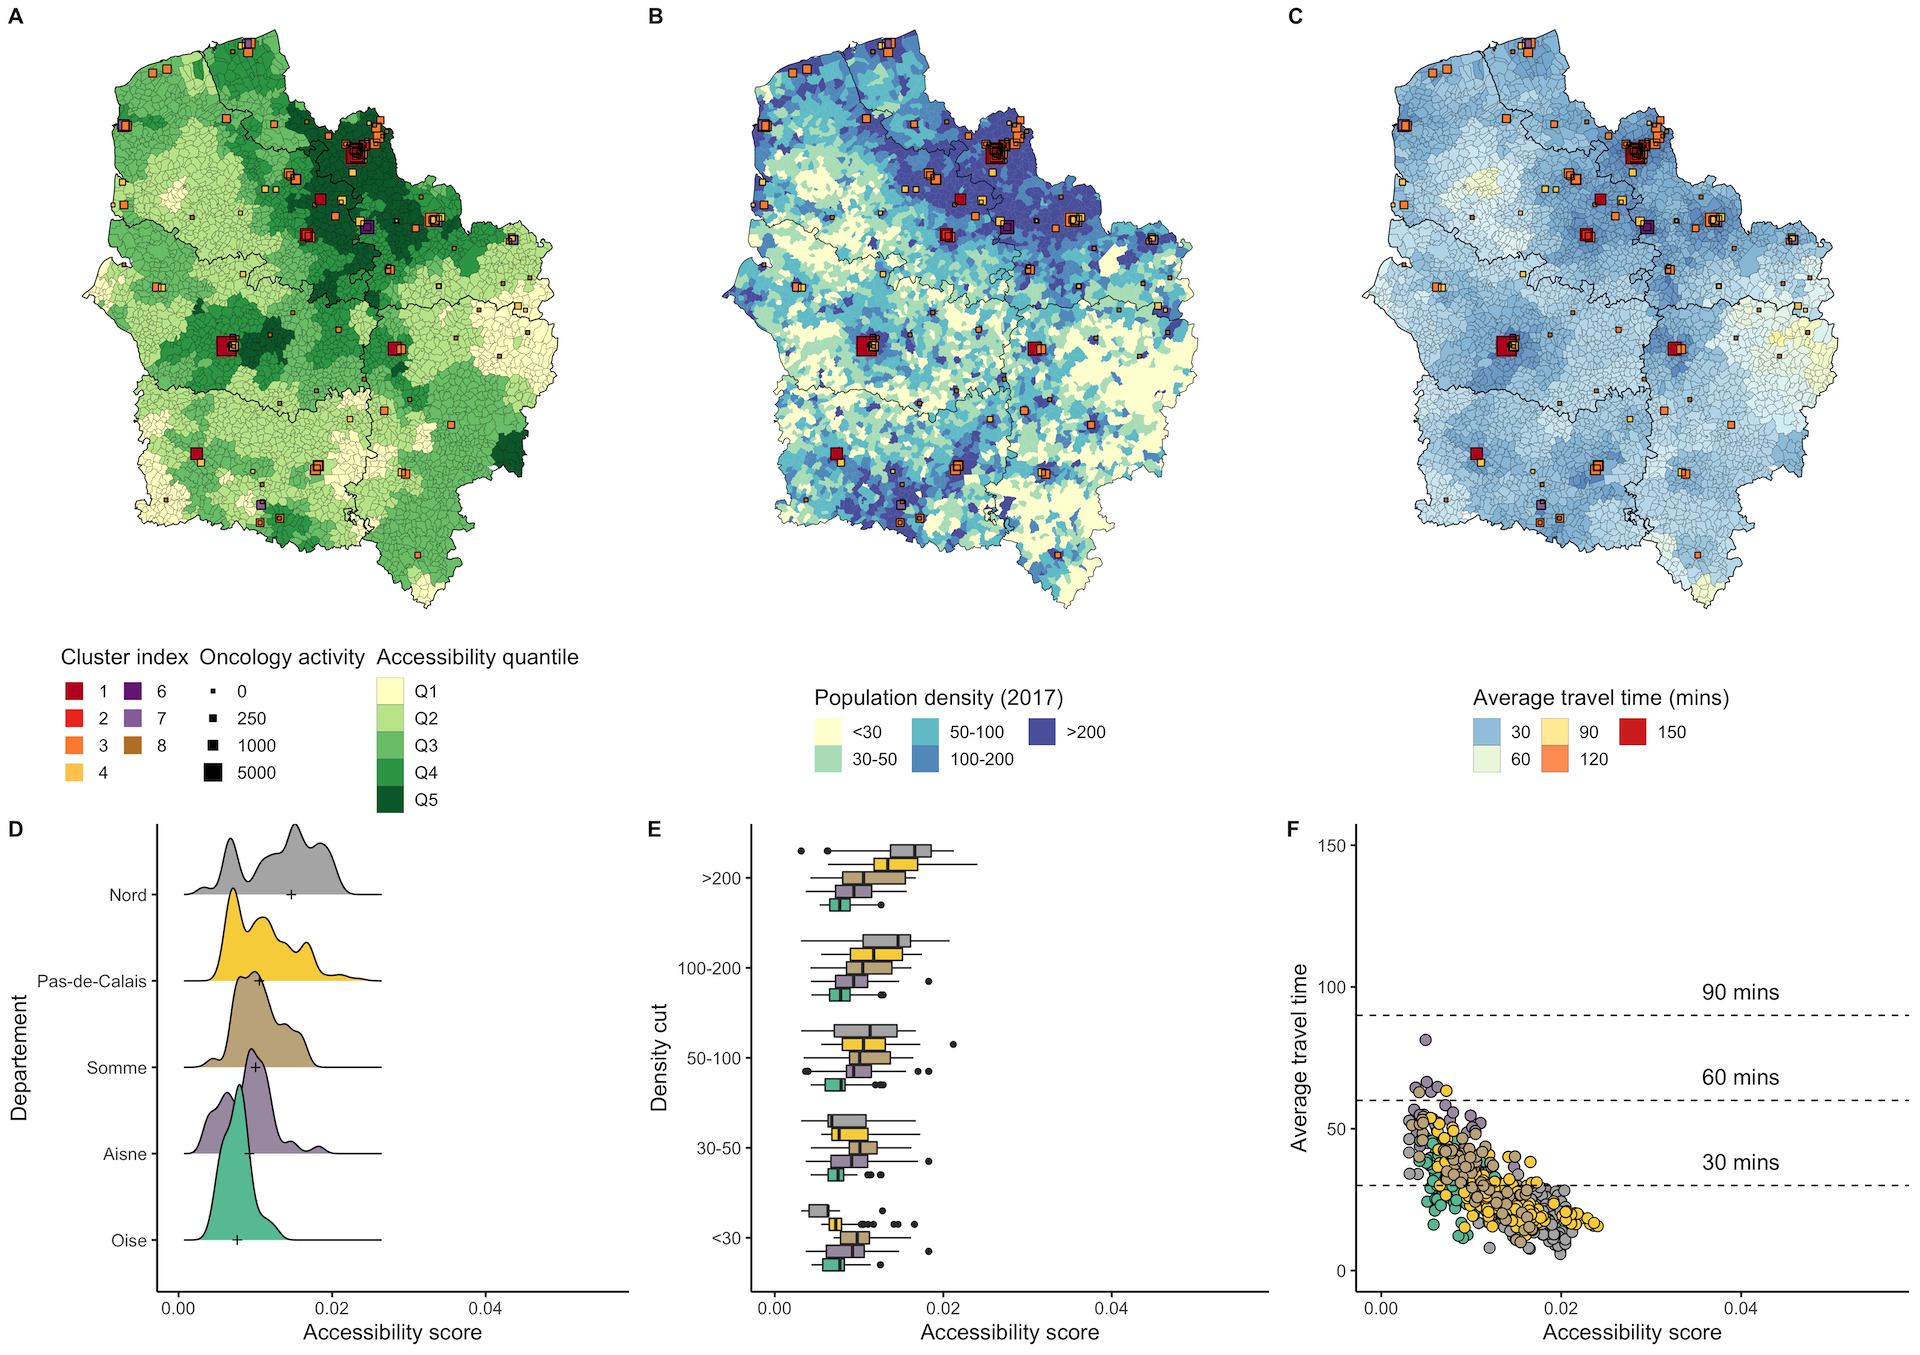
\includegraphics[width=0.9\textwidth]{images/camion/region_accessibility/accessibility_Hauts-de-France.png}
    \centering
    \caption{ \textbf{Accessibility distribution in Hauts-de-France.} The
        accessibility zones are relatively evenly distributed over the
        territory, although the best accessibility in this department is mainly
        in the urban and periurban area of Lille. Travel time averages 30
        minutes over most of the region, with the exception of the northern end
        of the region in the Aisne department and the northeastern part of the
        same department, where travel time averages 60 to 90 minutes }
\end{figure}

\subsection*{Accessibility in Grand Est region}

The Grand Est region is located in the east of France. It covers 57,433
km\textsuperscript{2} for a population of 5,556,219 (Insee) in 2019. 39\% of the
population resides in a rural commune (i.e., a commune with low or very low
density). 61\% of the population resides in urban areas, 22.8\% in peri-urban
rural areas and 16.2\% in autonomous rural areas, moreover nearly 80\% of the
regional surface is dedicated to agriculture and forestry. The Grand Est is
composed of 8 departments. The departments of Meuse and Haute-Marne central to
the region are among the most rural departments in France with respectively 74\%
and 67\% of their population living in rural areas (peri-urban and autonomous),
while the departments of Haut-Rhin, Bas-Rhin, Meurthe-et-Moselle and Moselle
have more than 60\% of their population living in urban areas (2018, Insee). The
department of Marne in the west of the region is home to Reims, the most densely
populated city in the region after Strasbourg.

The accessibility is high in the eastern half of the region in the departments
of Moselle, Meurthe et Moselle, Bas-Rhin, Haut-Rhin, particularly around the
large agglomerations (Strasbourg, Nancy, Metz, Colmar). Indeed, 41\% of the
population of the Grand Est is in an accessibility zone of Q5 and only 7.5\% in
a Q1 zone. The lack of accessibility in the western part of the region is more
pronounced due to the low or very low density areas that are more common in
these departments. Also, the link between population density and accessibility
is visible and reinforced by the consideration of average travel times. Travel
times are almost uniformly distributed over the entire territory, with little or
no travel time exceeding 30 minutes; travel times of 60 minutes on average are
limited and those of 90 minutes are very limited. These times are most prevalent
in the western half of the region in the very low density areas but mostly in
the less demographically dense areas.  The poor accessibility for the city of
Charles-Ville-Mézière (46,436 inhabitants in 2019) is more worrying in view of
its demographic density. However, it can be observed that the coverage of
maximum accessibility for the majority of the population does not necessarily
require a spatial accessibility spread over the surface of the region, since the
Grand Est has only 13.5\% of the surface of its territory considered as Q5
accessibility, but covers the needs of maximum accessibility for 41\ of its
population. Thus, the urban nature of the population of the Grand Est seems to
be a determining factor in maximizing accessibility to care.

\begin{figure}[h!]
    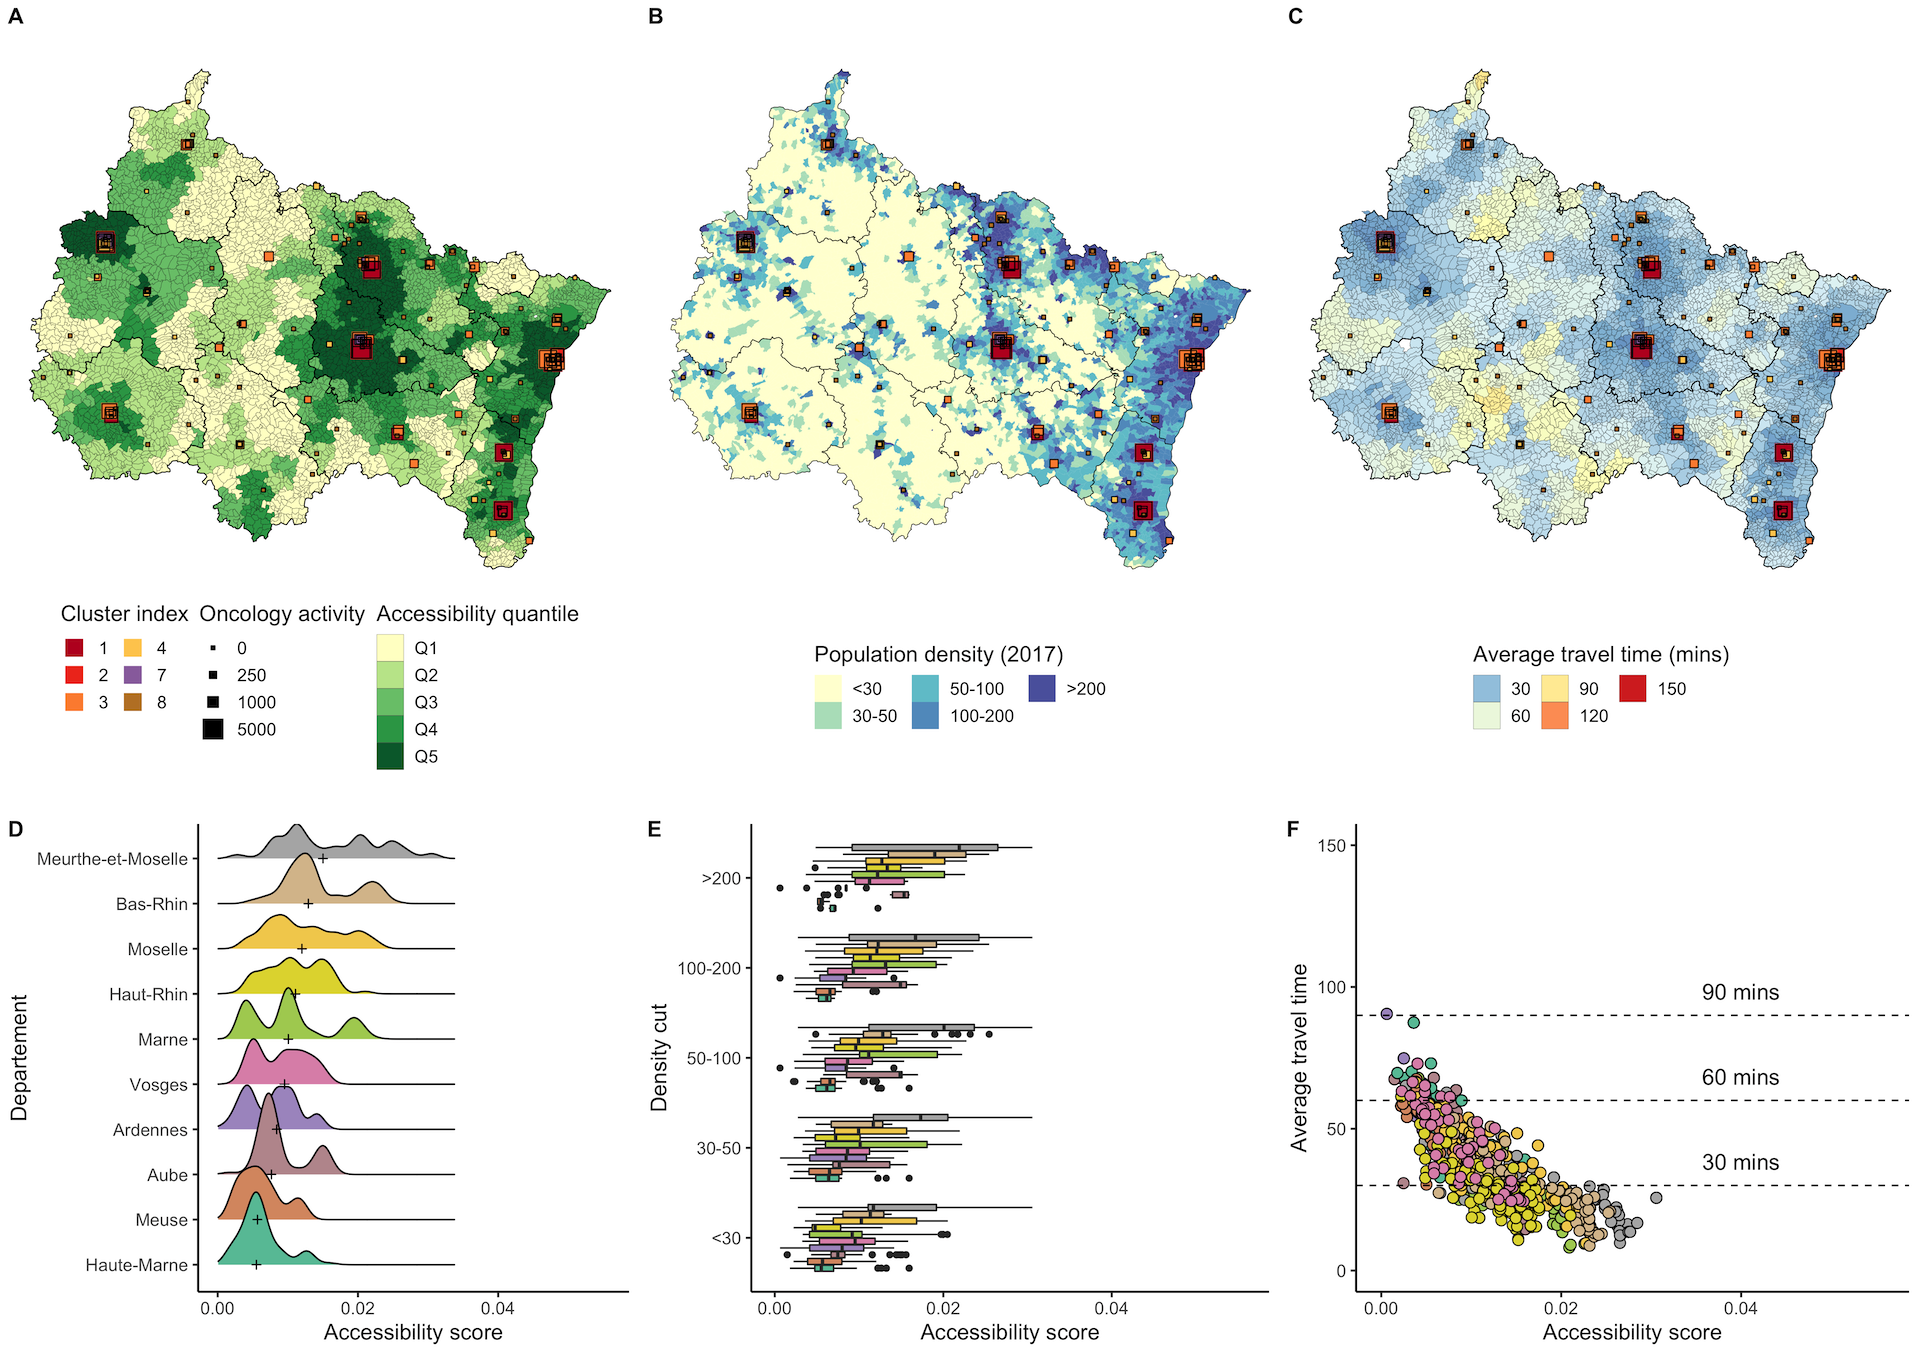
\includegraphics[width=0.9\textwidth]{images/camion/region_accessibility/accessibility_Grand-Est.png}
    \centering
    \caption{ \textbf{Accessibility distribution in Grand-Est.} We notice good
        accessibility scores in the eastern half of the region in the
        departments of Moselle, Meurthe et Moselle, Bas-Rhin, Haut-Rhin,
        particularly around the large agglomerations (Strasbourg, Nancy, Metz,
        Colmar). Indeed, 41\% of the population of the Grand Est is in an
        accessibility zone of Q5 and only 7.5\% in a Q1 zone. The lack of
        accessibility in the western part of the region is more pronounced due
        to the low or very low density areas that are more common in these
        departments. }
\end{figure}

\subsection*{Accessibility in Centre-Val de Loire region}

The Centre-Val-de-Loire region is located in the center west of France. It
covers an area of 39 151 km\textsuperscript{2} with a population of 2 573 180
(Insee) in 2019. The region is one of the most rural regions of France, with
90\% of its territory occupied by rural municipalities and 1 in 2 inhabitants
living in a rural municipality (49\%). 27\% of the population (700,000
inhabitants) live in a rural commune under the influence of a major pole and
nearly 22\% (of 570,000) outside the area of attraction of such a pole. However,
the CVdL includes two metropolitan areas, Orléans in the department of Loiret
and Tour in Indre-et-Loire, which together account for one-third of the regional
population. Paris also has an influence on the region, affecting 184,000
inhabitants under its influence, i.e., 7\% of the CVdL population. Thus, the
majority of the population (90\%) lives in an attractive urban area. The
Hauts-de-France is made up of 6 departments. The department of Indre-et-Loire
includes and Loiret includes the two metropolitan areas of the region Tour with
137,665 inhabitants and Orleans with 288,229 inhabitants in 2019.

The accessibility of the whole region is relatively lower than in other regions
observed so far. Many areas have a low or very low accessibility score despite a
medium population density. Areas with low or very low population density can
have a very low accessibility score, although low-density areas of the Cher have
a score around the Q3 quantile. Only the city of Tour and its vicinity shows a
maximum level of accessibility, as well as some surrounding parcel areas in the
department of Loir-et-Cher around the city of Blois and in the department of
Cher around Bourges. Even the city of Orleans has an accessibility score of Q4
despite the presence of level 1 clusters. The CVdL has the particularity of
being the only French region without a \ac{clcc} on its territory. The closest
\ac{clcc} are those in adjacent regions, in Paris in the Île-de-France and Anger
in Normandy. We can deduce that in order to access a specialized center, the
inhabitants of this region have to leave the region.  We can see that the level
1 clusters in the region are located in Tour, Orléans and Chartes. The
departments in the south of the region have lower level clusters, with the Cher
having only a level 3 and a level 7 cluster. This is reflected in the travel
times which are rather homogeneous and low in the northern and central
departments with average travel times of 30 minutes, while the southern
departments, Indre and Cher have much higher travel times throughout their
territory, around 60 minutes and 90 minutes.

\begin{figure}[h!]
    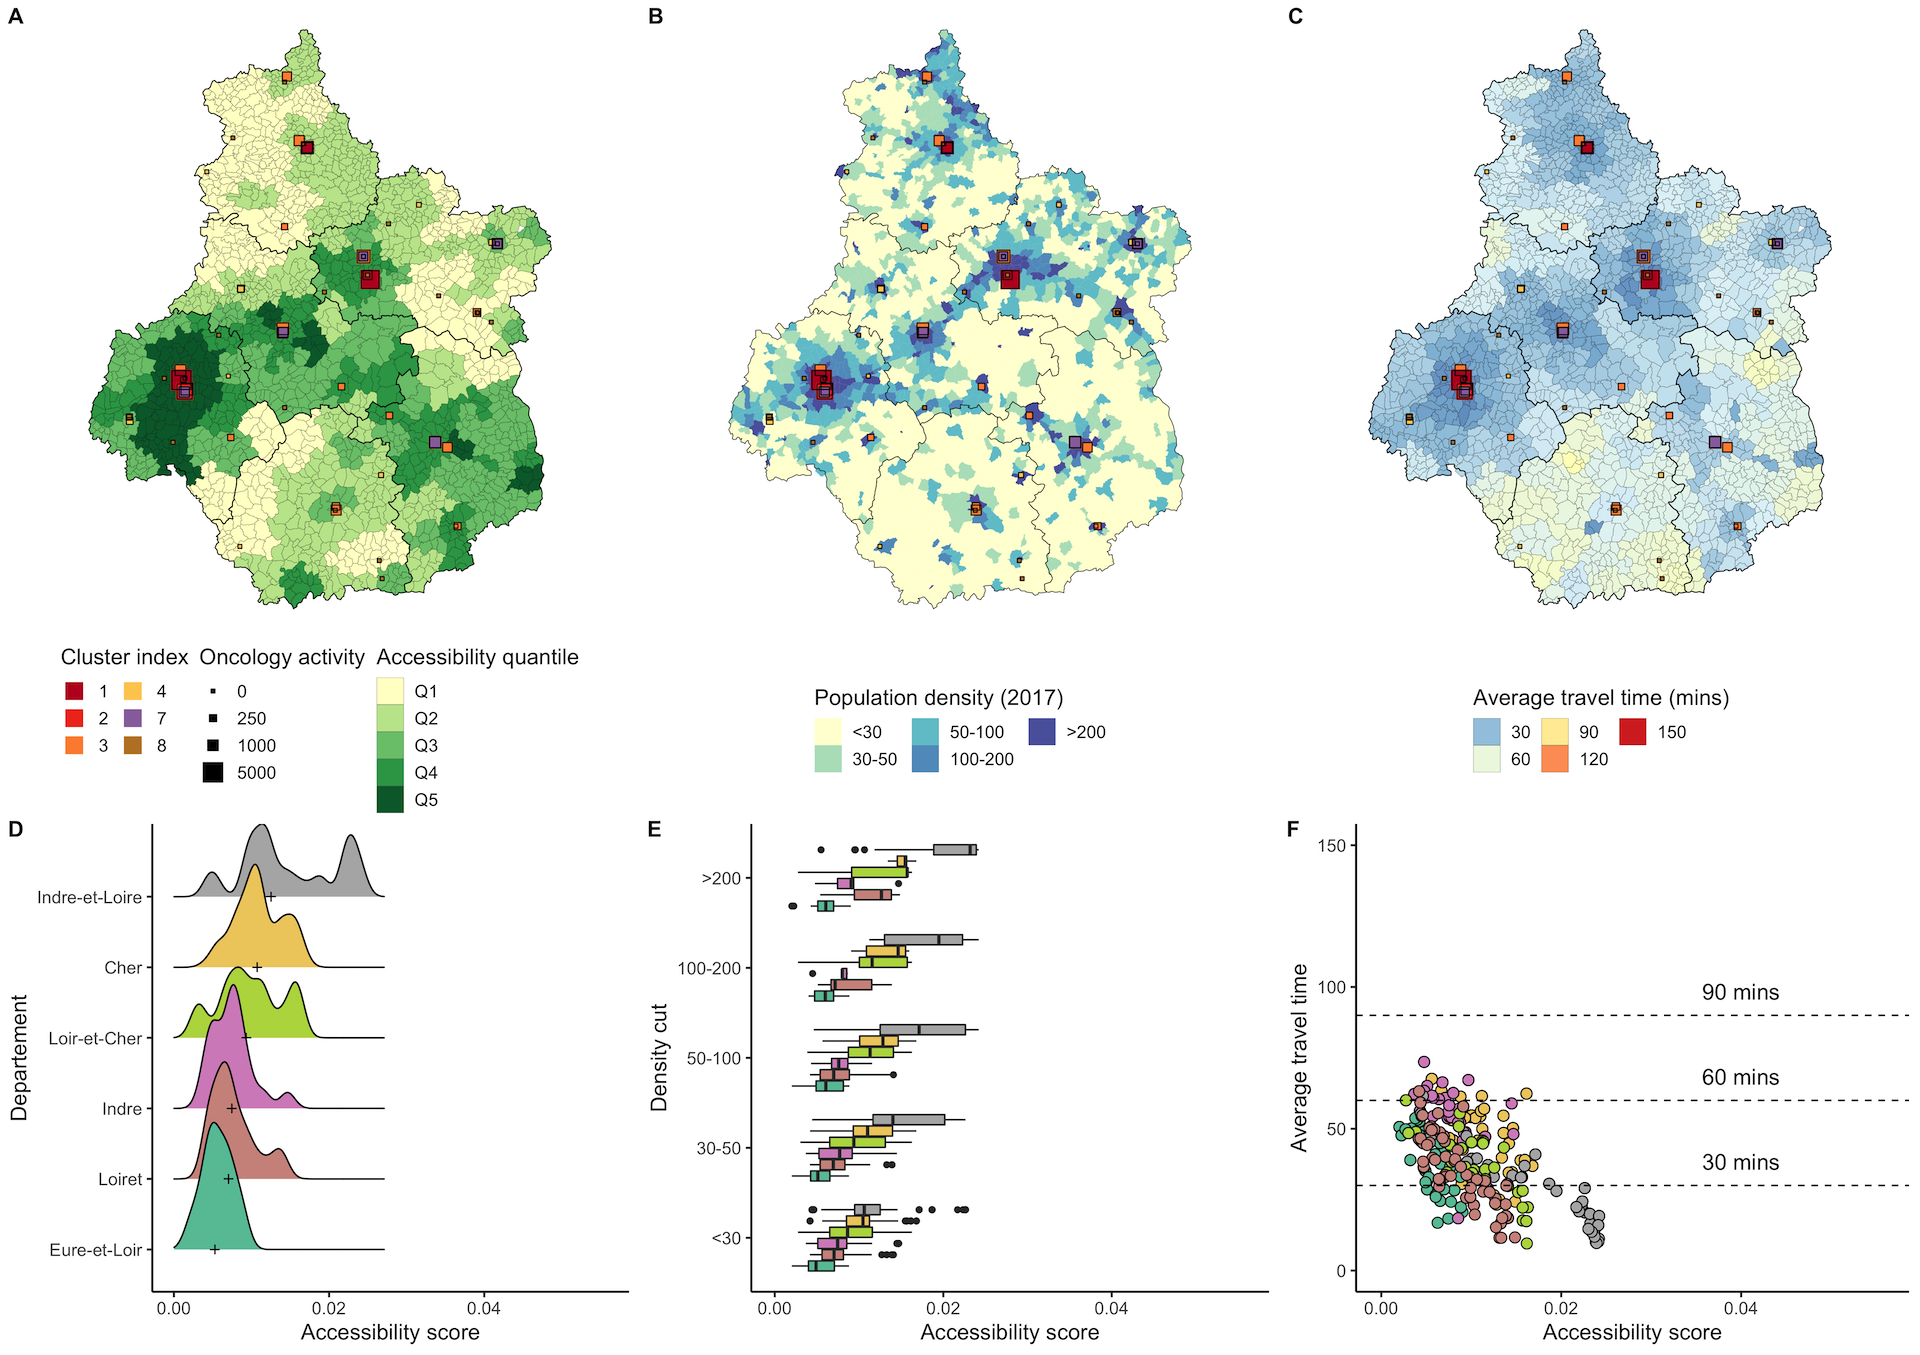
\includegraphics[width=0.9\textwidth]{images/camion/region_accessibility/accessibility_Centre-Val-de-Loire.png}
    \centering
    \caption{ \textbf{Accessibility distribution in Centre Val de Loire.} The
        accessibility of the whole region is relatively lower than in other
        regions observed so far. Many areas have a low or very low accessibility
        score despite a medium population density. Areas with low or very low
        population density can have a very low accessibility score, although
        low-density areas of the Cher have a score around the Q3 quantile. Only
        the city of Tour and its vicinity shows a maximum level of
        accessibility, as well as some surrounding parcel areas in the
        department of Loir-et-Cher around the city of Blois and in the
        department of Cher around Bourges. }
\end{figure}

\subsection*{Accessibility in Bretagne region}

The region of Bretagne is located in the west of France, on the Atlantic coast.
It covers 27,208 km², making it the largest region in France, with a population
of 3,354,854 (Insee) in 2019. More than half of the Breton population (53.7\%)
resides in a rural commune, so Bretagne is the second most rural region of
metropolitan France after Burgundy-Franche-Comté. The Breton rural area is
characterized by longer travel times to everyday services. 25.7\% of the
inhabitants of very sparsely populated autonomous areas have to travel more than
10 minutes on average to access them, and for 68.6\% of them, the average
journey takes between 7 and 10 minutes. However, a major part of the population
lives in an attractive urban area, i.e. 87\% of the region's population.
Bretagne is composed of 5 departments. The main metropolis of the region is
Rennes with 215,366 inhabitants and 364,133 inhabitants in its urban unit, the
first agglomeration of the department of Ille-et-Vilaine, followed by Brest
which is located in the department of Finistère with 139,926 inhabitants.

Bretagne has very good accessibility with 57.7\% of its population living in a
territory with maximum accessibility and above all a very low rate of its
population in territories with low or very low accessibility with 5.1\% of its
population in Q2 and only 1.5\% of its population in Q1. Also, the maps show a
good distribution of accessibility throughout the territory, with variations
often related to the territory's population density ratio. Travel times reflect
the level of accessibility, with many travel times less than 30 minutes and some
travel times between 30 and 60 minutes but very rarely more. However, Morbihan
has a relatively high proportion of trips between 30 and 60 minutes, including
rare areas where travel times exceed 90 minutes, particularly due to the
department's profile, which includes certain islands such as Belle-Île, which
have travel times of over 120 minutes.


\begin{figure}[h!]
    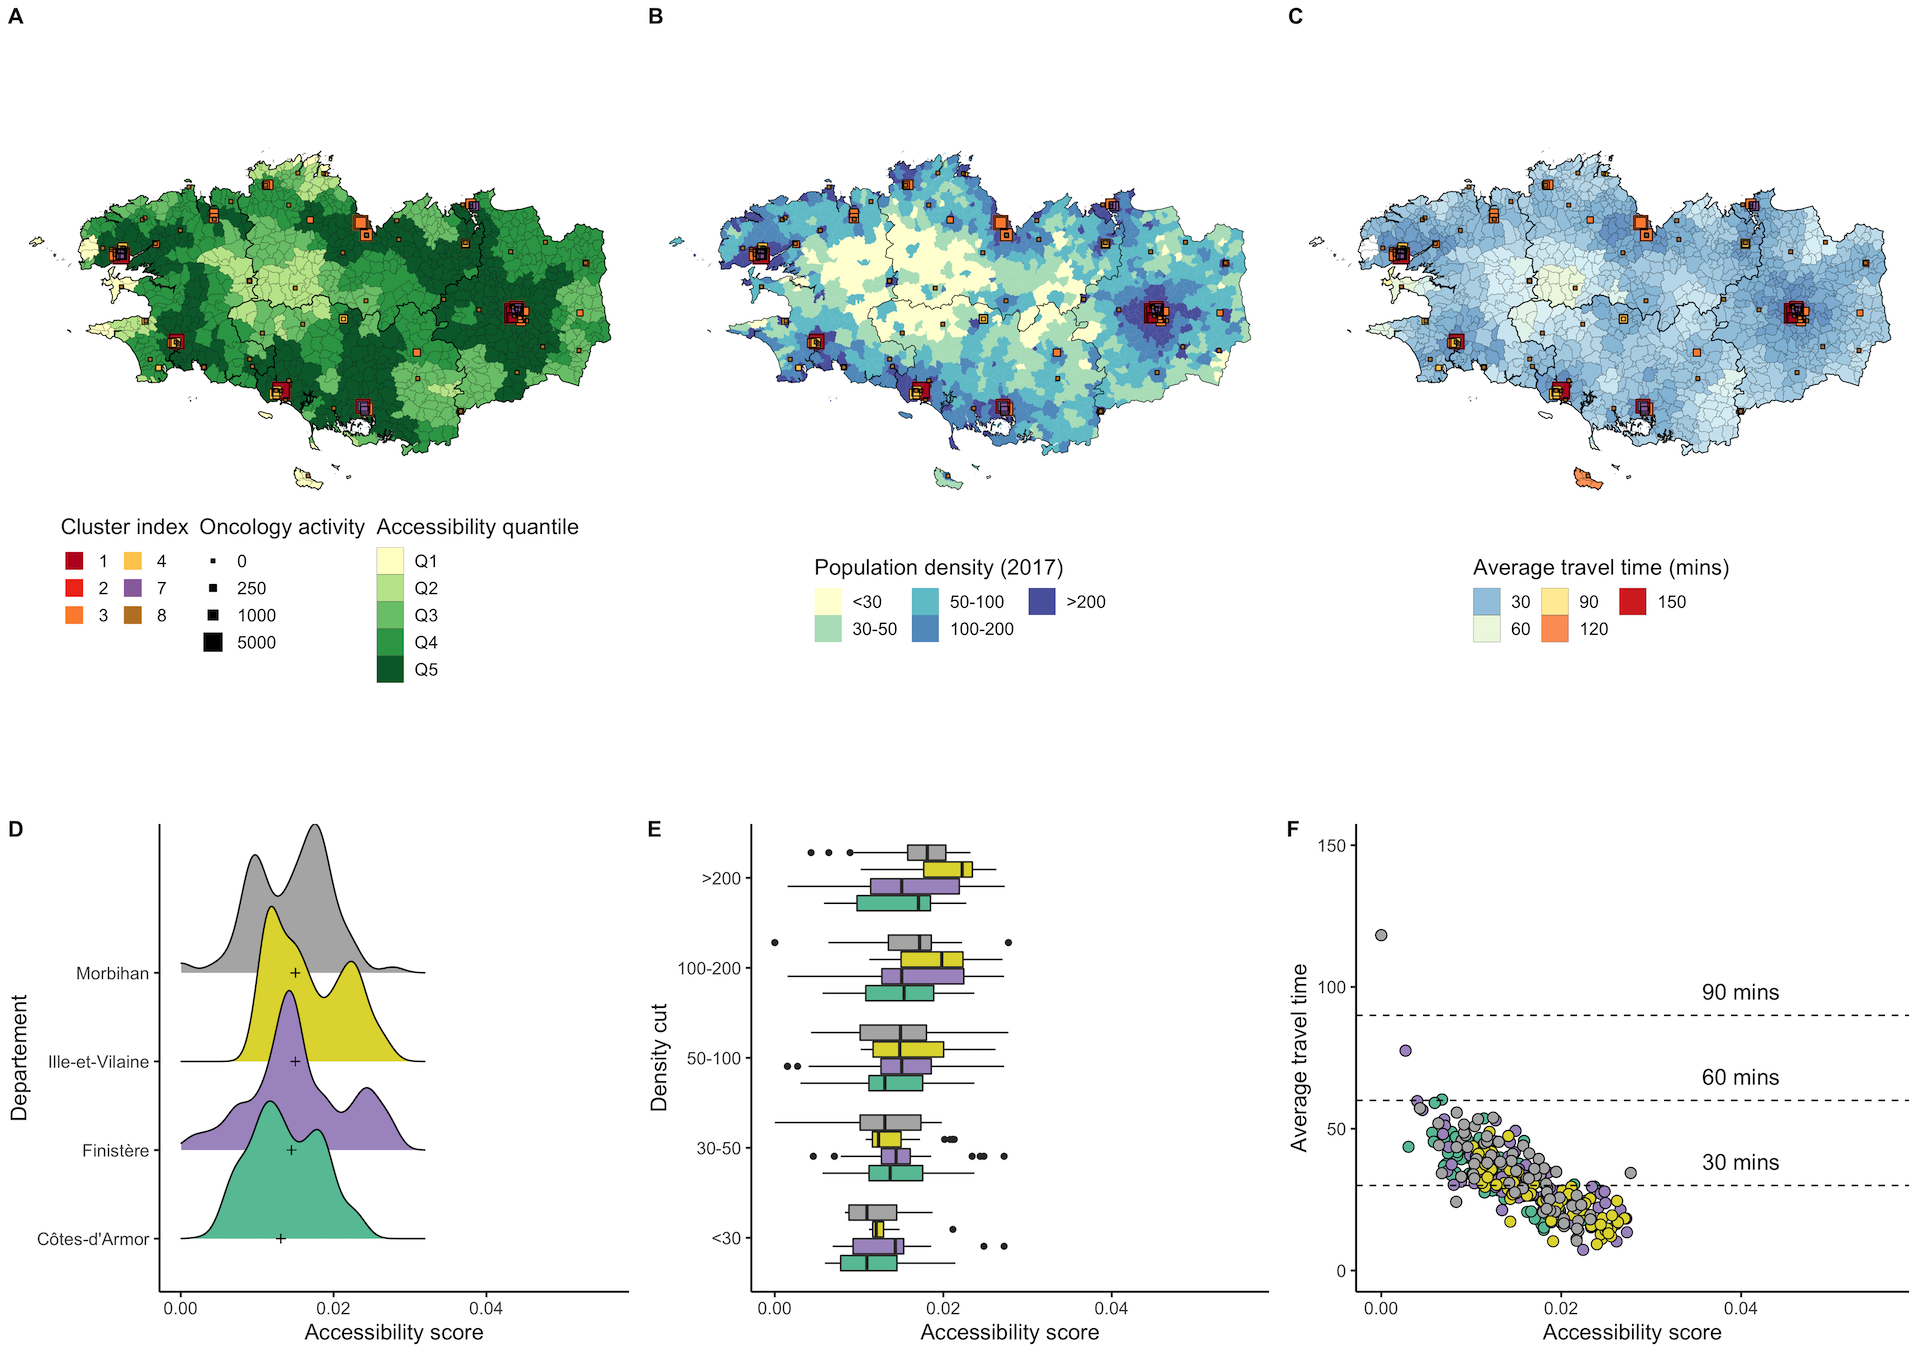
\includegraphics[width=0.9\textwidth]{images/camion/region_accessibility/accessibility_Bretagne.png}
    \centering
    \caption{
        \textbf{Accessibility distribution in Bretagne.}
    }
\end{figure}

\subsection*{Accessibility in Bourgogne-Franche-Comté region}

The Bourgogne-Franche-Comté (BFC) region is located in the center-east of
France. It covers 47,784 km\textsuperscript{2} for a population of 2,805,580
(Insee) in 2019 with 1,242,882 active people. In 2018 the BFC is considered the
first rural region of France with more than half of its population (1.5 million
people) residing in rural areas. The BFC is composed of 8 departments. The
departments of Yvonne, Nièvre to the west, Saône-et-Loire and Jura to the south,
have a particularly rural and agricultural landscape without dense urban areas,
especially for Saône-et-Loire.  In the department of Côte-d'Or is located Dijon,
the largest and most densely populated city in the region with 158,002
inhabitants, ahead of the city of Besançon with its 117,912 inhabitants, which
is located to the east in the department of Doub. In total, the BFC region has
3,704 municipalities, 26 of which have more than 10,000 inhabitants.

The departments of Côte-d'Or and Doubs have the best accessibility, especially
around densely populated urban areas such as Dijon or Besançon. Some areas of
the region have a low accessibility quantile Q1 and Q2 which cover 37.3\% and
16.4\% respectively of the regional territory, i.e. more than half (53.7\%) of
the area is recognized with a level of accessibility to cancer care. The areas
with low or very low accessibility are located mainly in rural areas and with
low or very low population density, except for the eastern border of the Doubs,
which has more densely populated areas, but with more mountainous terrain, with
a quantile 1 accessibility. In each department, accessibility is best in the
urban areas and their surroundings. The travel time shows an unequal
distribution of access to health care in the territory, since the majority of
municipalities have an average travel time of 30 minutes, but large areas of the
region show average travel times of 60 or 90 minutes, particularly in the
departments of Nièvre and Yvonne, although in the less densely populated areas
of these departments, or travel times exceeding 120 minutes in the east of the
Jura at the Swiss border, which is, however, likely to be a more mountainous
terrain

\begin{figure}[h!]
    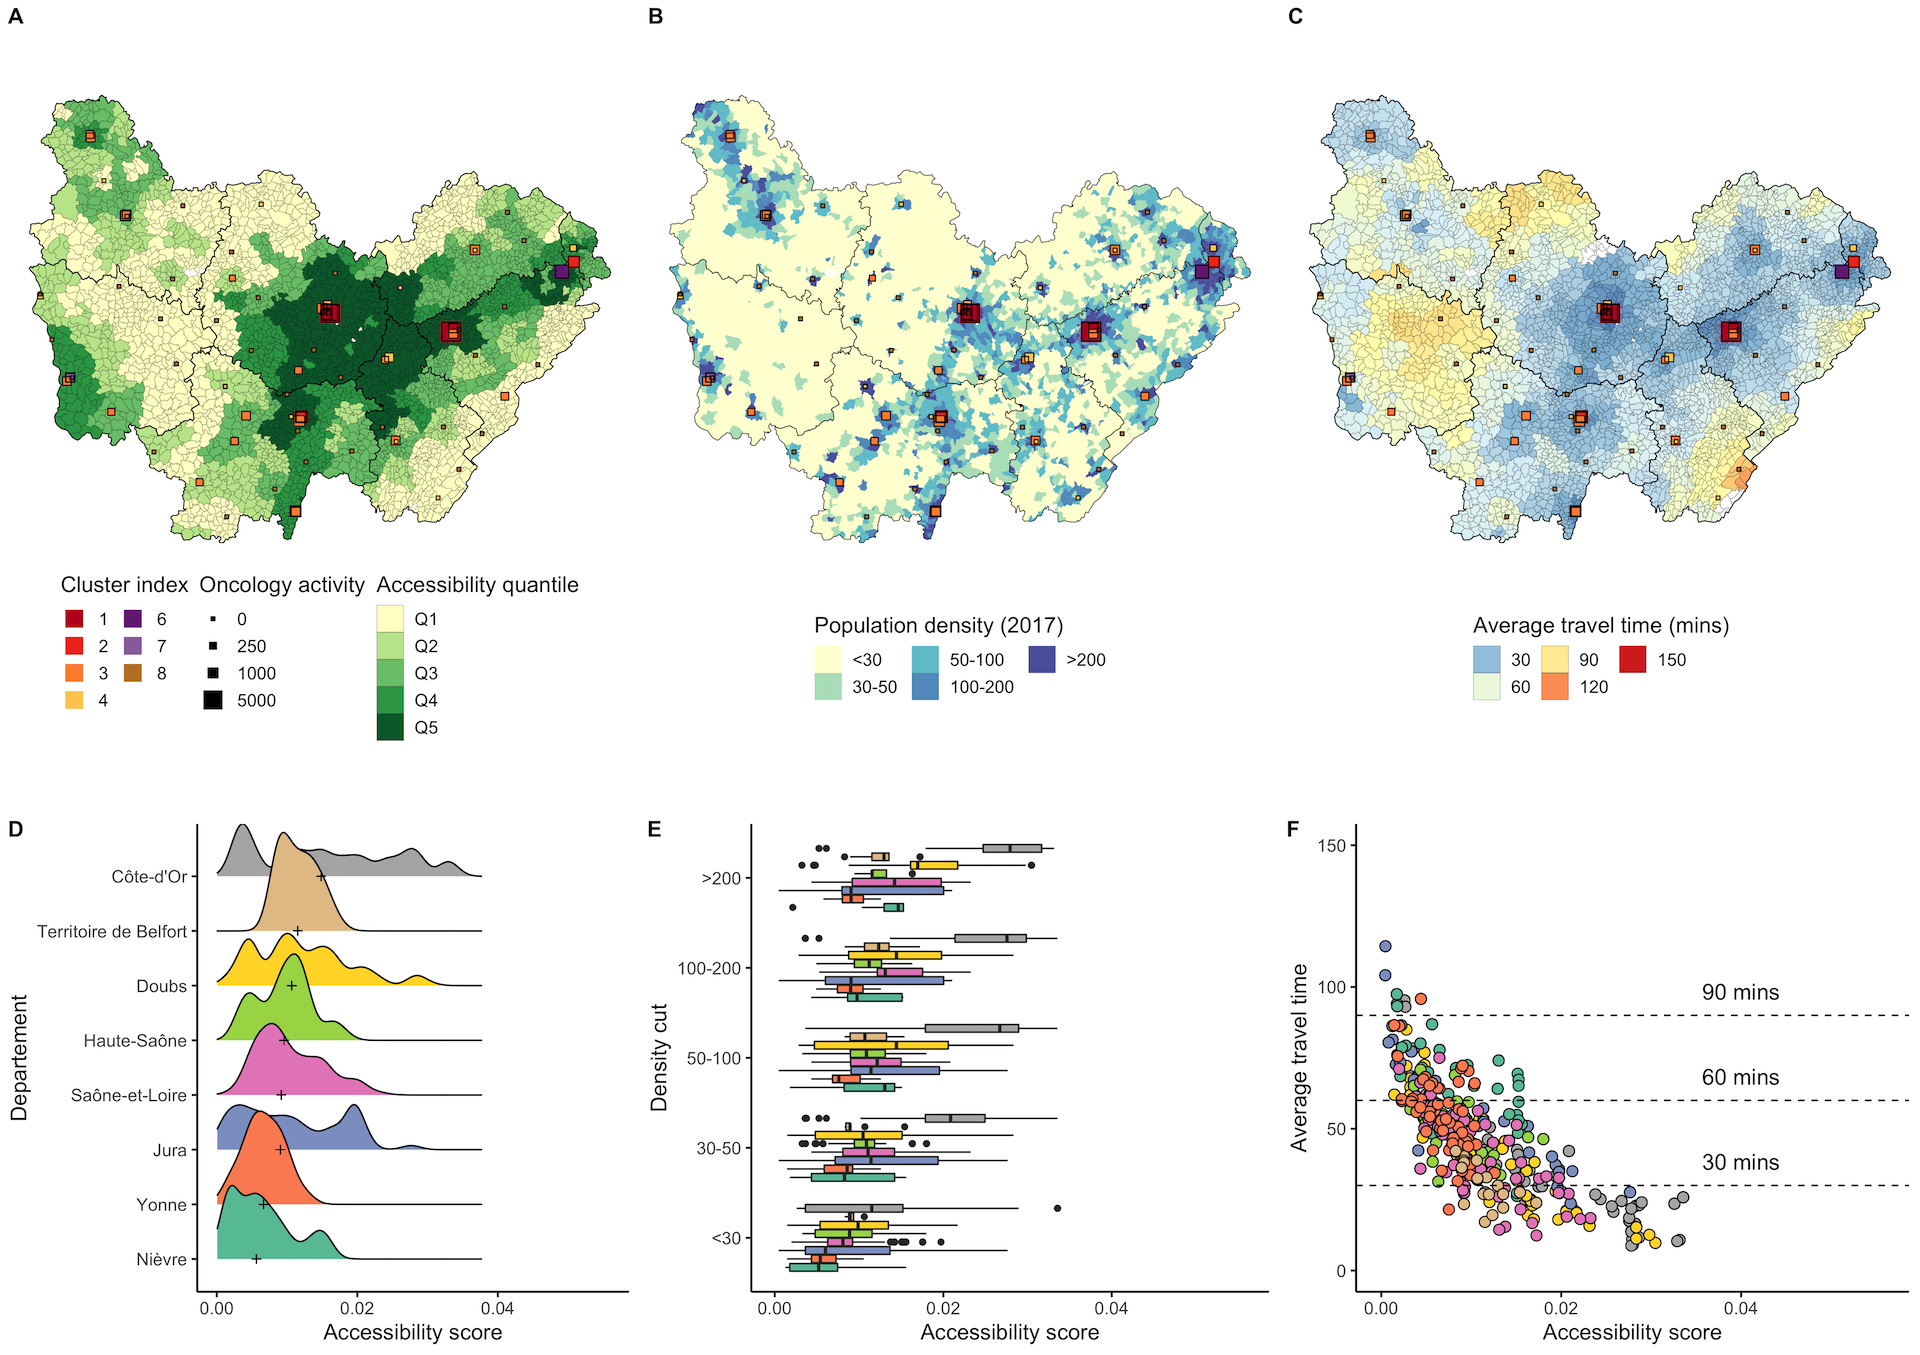
\includegraphics[width=0.9\textwidth]{images/camion/region_accessibility/accessibility_Bourgogne-Franche-Comte.png}
    \centering
    \caption{ \textbf{Accessibility distribution in Bourgogne-Franche-Comté.}
        The departments of Côte-d'Or and Doubs have the best accessibility,
        especially around densely populated urban areas such as Dijon or
        Besançon. Some areas of the region have a low accessibility quantile Q1
        and Q2 which cover 37.3\% and 16.4\% respectively of the regional
        territory, i.e. more than half (53.7\%) of the area is recognized with a
        level of accessibility to cancer care. The areas with low or very low
        accessibility are located mainly in rural areas and with low or very low
        population density, except for the eastern border of the Doubs, which
        has more densely populated areas, but with more mountainous terrain,
        with a quantile 1 accessibility. }
\end{figure}

\subsection*{Accessibility in Auvergne-Rhône-Alpes region}

The Auvergne-Rhône-Alpes (ARA) region is located in eastern France. It covers
69,711 km\textsuperscript{2} for a population of 7,994,459 (Insee) in 2018,
representing 12.3\% of the metropolitan population, i.e. the most populated
region in France. The ARA is the main mountain region of France with 2.2 million
people residing in a municipality classified as a mountain area, with more than
half in the regional part of the Massif Central which is distributed in a
diagonal of low population density, while the population of the Alpine massif is
concentrated in the urbanized and more densely populated parts at the bottom of
valleys. In the ARA, 35\% of the population lives in a rural commune, the
provincial metropolitan average being 33\%, and these communes cover 89\% of the
region's surface area. The ARA is composed of 12 departments. The Rhône
department in the northern center of the region includes the city of Lyon, the
second largest city in France, which has 1,411,571 inhabitants in its
metropolis. The eastern departments, Savoie, Haute-Savoie, Isère, Drôme,
constitute the mountainous areas of the region. Of the twelve departments, five
are considered 'essentially rural': Cantal (74\% of the inhabitants live in
rural communes), Haute-Loire (70\%), Ardèche (60\%), Allier (58\%) and Ain
(50\%).

If we look at the maps, we can see that the areas with the lowest accessibility
are mainly located in areas with low or very low density, particularly along the
mountainous border in the east of the region in the departments of Haute-Savoie,
Savoie, Isère and Drôme. It is possible to observe a good distribution of
accessibility in the central, northern and north-western part of the region,
particularly around the large agglomerations such as the city of Lyon,
Clermont-Ferrand, Moulins, Grenoble and Aurillac. The three southern
departments, Haute-Loire, Ardèche and Drôme, are less accessible than the other
departments in the region. Above all, it can be observed that the mountainous
terrain tends to have a strong impact on accessibility to care, since travel
times in these areas, particularly for the departments of Drôme and Savoie,
reach an average of 120 minutes if not 150 minutes. In the mountainous
departments of the east, the valleys that contain the urban centers with the
highest population density, such as Chambéry, Grenoble and Annecy, are the most
favorable accessibility centers in these departments. Despite its mountainous
nature, 51.1\% of the Auvergne-Rhône-Alpes region is located in an accessibility
zone Q5 compared to 8\% in an accessibility zone Q1.

\begin{figure}[h!]
    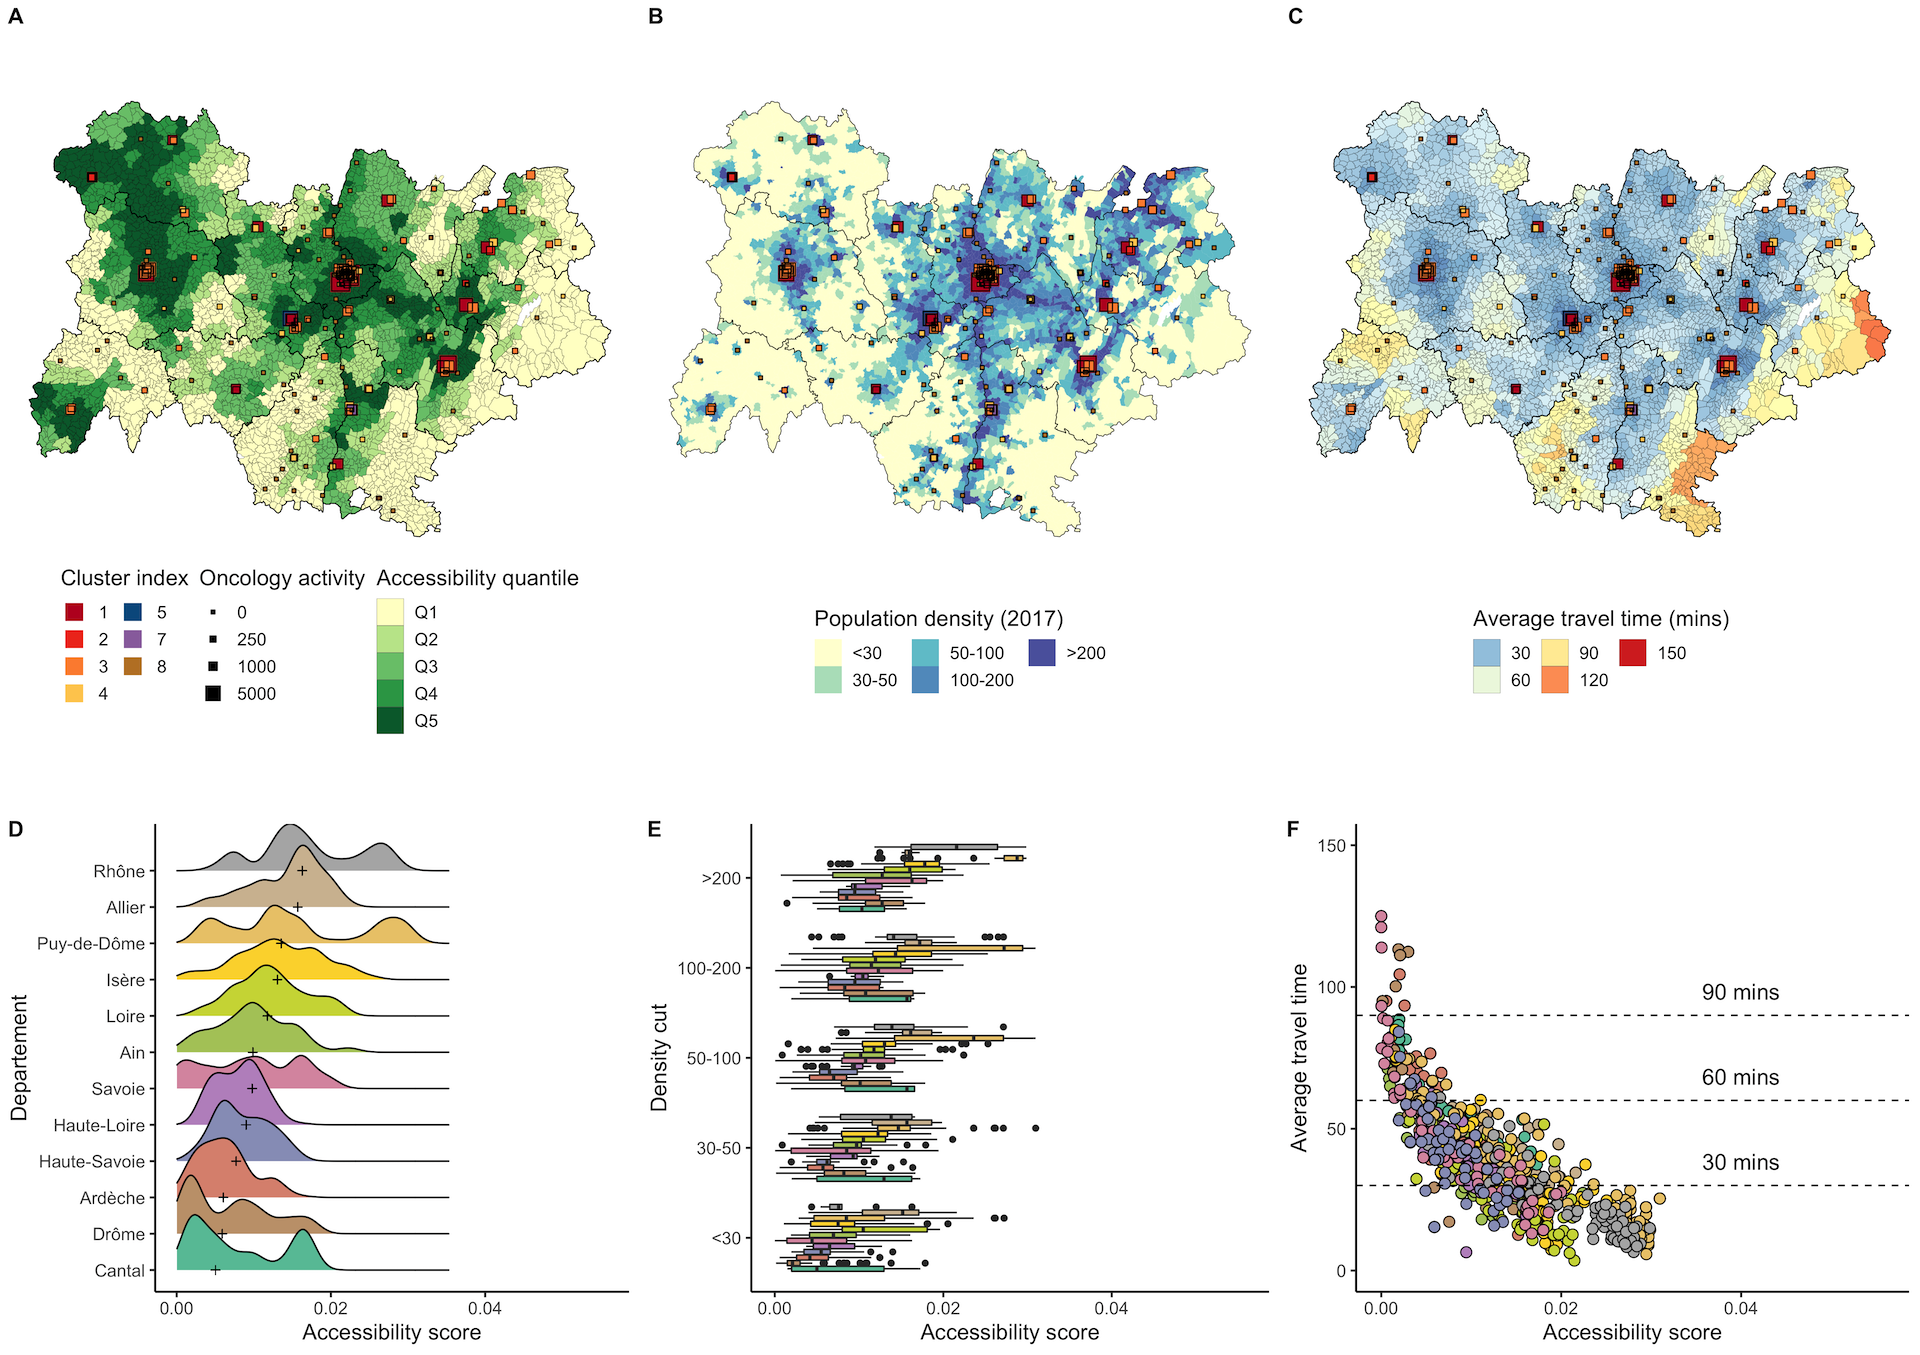
\includegraphics[width=0.9\textwidth]{images/camion/region_accessibility/accessibility_Auvergne-Rhone-Alpes.png}
    \centering
    \caption{ \textbf{Accessibility distribution in Auvergne-Rhone-Alpes.} The
        areas with the lowest accessibility are mainly located in areas with low
        or very low density, particularly along the mountainous border in the
        east of the region in the departments of Haute-Savoie, Savoie, Isère and
        Drôme. It is possible to observe a good distribution of accessibility in
        the central, northern and north-western part of the region, particularly
        around the large agglomerations such as the city of Lyon,
        Clermont-Ferrand, Moulins, Grenoble and Aurillac. The three southern
        departments, Haute-Loire, Ardèche and Drôme, are less accessible than
        the other departments in the region. Above all, it can be observed that
        the mountainous terrain tends to have a strong impact on accessibility
        to care, since travel times in these areas, particularly for the
        departments of Drôme and Savoie, reach an average of 120 minutes if not
        150 minutes. }
\end{figure}

\section{Conclusion}

In this section, we described our method to compute the oncology accessibility
score given to every municipality in metropolitan France. This score was
obtained by using the \acf{e2sfca} algorithm, with oncology activity as supply,
municipality population as demand, and driving car duration as impedance metric.
Specific attention should be given to municipalities with very poor access to
oncology care centers. While we saw that most of the population lives in high
accessibility areas, around 6\% of the population lives in the bottom 20\%
accessibility quantile. Among these municipalities, some are very rural and
mountainous like those in the Alpes-de-Haute-Provence in
Provence-Alpes-Cote-d'Azur region. Such areas cannot be expected to have a very
good healthcare coverage. By contrast, the case of suburban areas with
relatively dense population and poor accessibility should be addressed more
easily. Our optimization algorithm can help driving public health policies, as
it effectively identifies areas where accessibility could grow, by allocating
additional oncology activity to a restricted number of care centers. The
proposed growth factors are indicative and do not have to be effective within a
year, as it represents a considerable effort for care centers to increase their
activity. Our oncology accessibility score is deliberately non-specific to
cancer type. This score is meant to outline how easy it would be for a
population location to reach a first entry point for oncology care. Here, we are
only focusing on surgery, chemotherapy, and radiotherapy treatments. The same
technique could be used on a specific cancer type, the method will remain the
same, only the supply variable used in the accessibility score will change. We
should mention that \ac{sa} is better suited for pathologies that are relatively
well handled across the whole country. Accessibility for rare diseases like
pediatric cancer or complex cancers that re-quire a specific expertise is less
informative because only a handful of care centers are indicated. Similarly, we
could compute an accessibility score that is focused on specific kinds of stays:
our web application lets the user pick between surgery, chemotherapy, or
radiotherapy as supply variable.
